\documentclass[12pt,a4paper]{report}
\usepackage[utf8]{inputenc}
\usepackage[T1]{fontenc}
\usepackage[margin=1in]{geometry}
\usepackage{graphicx}
\usepackage{hyperref}
\usepackage{setspace}
\usepackage{float}
\usepackage{booktabs}
\usepackage{longtable}
\usepackage{array}
\usepackage{multirow}
\usepackage{listings}
\usepackage{xcolor}
\usepackage{fancyhdr}
\usepackage{amsmath}
\usepackage{parskip}
% Standard enumerate used throughout

% Hyperref setup
\hypersetup{
    colorlinks=true,
    linkcolor=blue,
    urlcolor=blue,
    citecolor=blue,
    pdftitle={AI-Based Real-Time eKYC System for Deepfake-Free Identity Verification},
    pdfauthor={Hardik Sharma}
}

% Code listing style
\lstdefinestyle{pythonstyle}{
    language=Python,
    basicstyle=\ttfamily\footnotesize,
    keywordstyle=\color{blue}\bfseries,
    commentstyle=\color{gray},
    stringstyle=\color{orange},
    showstringspaces=false,
    breaklines=true,
    frame=single,
    numbers=left,
    numberstyle=\tiny\color{gray},
    tabsize=4,
    captionpos=b
}

\lstdefinestyle{tsstyle}{
    language=Java,
    basicstyle=\ttfamily\footnotesize,
    keywordstyle=\color{blue}\bfseries,
    commentstyle=\color{gray},
    stringstyle=\color{orange},
    showstringspaces=false,
    breaklines=true,
    frame=single,
    numbers=left,
    numberstyle=\tiny\color{gray},
    tabsize=2,
    captionpos=b
}

\lstdefinestyle{sqlstyle}{
    language=SQL,
    basicstyle=\ttfamily\footnotesize,
    keywordstyle=\color{blue}\bfseries,
    commentstyle=\color{gray},
    stringstyle=\color{orange},
    showstringspaces=false,
    breaklines=true,
    frame=single,
    numbers=left,
    numberstyle=\tiny\color{gray},
    tabsize=4,
    captionpos=b
}

% Header/Footer
\pagestyle{fancy}
\fancyhf{}
\fancyhead[L]{\small AI-Based Real-Time eKYC System}
\fancyhead[R]{\small Hardik Sharma -- 2353777736}
\fancyfoot[C]{\thepage}
\setlength{\headheight}{15pt}


\setstretch{1.4}
\setlength{\parskip}{0.5em}

\graphicspath{{./04_diagrams/rendered/}{./04_diagrams/approved_synopsis/}}

\begin{document}

% =====================================================================
%  TITLE PAGE
% =====================================================================
\begin{titlepage}
    \centering
    \vspace*{0.5cm}

    {\Large \textbf{INDIRA GANDHI NATIONAL OPEN UNIVERSITY}}\\[0.3cm]
    {\large School of Computer and Information Sciences}\\[0.2cm]
    {\large Maidan Garhi, New Delhi -- 110068}\\[1cm]

    \rule{\textwidth}{1.5pt}\\[0.4cm]
    {\LARGE \textbf{MCSP-232 PROJECT REPORT}}\\[0.4cm]
    \rule{\textwidth}{1.5pt}\\[1.2cm]

    {\LARGE \textbf{AI-Based Real-Time eKYC System for\\[0.3cm]
    Deepfake-Free Identity Verification}}\\[2cm]

    \begin{flushleft}
    \large
    \textbf{Submitted by:}\\[0.2cm]
    Hardik Sharma\\
    Enrolment No: 2353777736\\
    Programme: MCA (MCAOL)\\[0.8cm]

    \textbf{Under the Guidance of:}\\[0.2cm]
    Anshul Sharma\\
    AI Engineer\\
    IDS Infotech Ltd., Chandigarh\\[1cm]
    \end{flushleft}

    \vfill
    {\large \textbf{July 2025}}

\end{titlepage}

% =====================================================================
%  CERTIFICATE
% =====================================================================
\newpage
\thispagestyle{empty}
\begin{center}
    {\Large \textbf{CERTIFICATE}}
\end{center}
\vspace{1cm}

This is to certify that the project report entitled \textbf{``AI-Based Real-Time eKYC System for Deepfake-Free Identity Verification''} submitted to Indira Gandhi National Open University in partial fulfilment of the requirements for the award of the degree of \textbf{Master of Computer Applications (MCA)} is an authentic record of bonafide work carried out by \textbf{Mr.~Hardik Sharma} (Enrolment No.~\textbf{2353777736}) under my guidance and supervision.

The matter embodied in this report has not been submitted for the award of any other degree or diploma to this University or any other institution.

\vspace{2cm}

\begin{minipage}[t]{0.45\textwidth}
    \rule{6cm}{0.5pt}\\
    \textbf{Signature of Supervisor}\\[0.4cm]
    \textbf{Name:} Anshul Sharma\\
    \textbf{Designation:} AI Engineer\\
    \textbf{Organization:} IDS Infotech Ltd.\\
    \textbf{Date:} \underline{\hspace{3cm}}
\end{minipage}
\hfill
\begin{minipage}[t]{0.45\textwidth}
    \rule{6cm}{0.5pt}\\
    \textbf{Signature of Student}\\[0.4cm]
    \textbf{Name:} Hardik Sharma\\
    \textbf{Enrolment No:} 2353777736\\
    \textbf{Date:} \underline{\hspace{3cm}}
\end{minipage}

\vspace{2cm}
\begin{center}
    \rule{6cm}{0.5pt}\\
    \textbf{Signature of Coordinator / Study Centre}\\[0.3cm]
    \textbf{Date:} \underline{\hspace{3cm}}
\end{center}

% =====================================================================
%  DECLARATION
% =====================================================================
\newpage
\thispagestyle{empty}
\begin{center}
    {\Large \textbf{DECLARATION}}
\end{center}
\vspace{1cm}

I, \textbf{Hardik Sharma}, Enrolment No.~\textbf{2353777736}, a student of Master of Computer Applications (MCA) at Indira Gandhi National Open University, hereby declare that the project work presented in this report entitled \textbf{``AI-Based Real-Time eKYC System for Deepfake-Free Identity Verification''} has been carried out by me under the supervision of Mr.~Anshul Sharma, AI Engineer, IDS Infotech Ltd., Chandigarh.

I declare that:
\begin{enumerate}
    \item This work is entirely my own and has not been submitted to any other university or institution for the award of any degree or diploma.
    \item All information, data, facts and figures presented in this report are correct to the best of my knowledge.
    \item I have acknowledged all sources of information and have cited them appropriately wherever they have been used.
    \item I understand that any falsification or plagiarism is a serious academic offence and may result in cancellation of the degree.
\end{enumerate}

\vspace{2cm}

\begin{flushleft}
\rule{6cm}{0.5pt}\\
\textbf{Hardik Sharma}\\
Enrolment No: 2353777736\\
MCA (MCAOL), IGNOU\\
Date: \underline{\hspace{3cm}}
\end{flushleft}

% =====================================================================
%  ACKNOWLEDGEMENTS
% =====================================================================
\newpage
\thispagestyle{empty}
\begin{center}
    {\Large \textbf{ACKNOWLEDGEMENTS}}
\end{center}
\vspace{0.5cm}

I am grateful to all who contributed to the successful completion of this project.

I express my sincere gratitude to my project supervisor \textbf{Mr.~Anshul Sharma}, AI Engineer at IDS Infotech Ltd., Chandigarh, for his invaluable guidance, constant encouragement, and constructive feedback throughout the development of this system. His expertise in artificial intelligence and practical industry insights were indispensable in shaping both the technical direction and the quality of this work.

I would like to thank the \textbf{School of Computer and Information Sciences, IGNOU}, for providing this learning opportunity through the MCSP-232 project course and for the structured guidelines that helped me plan and execute the project systematically.

I am deeply thankful to the open-source community -- particularly the contributors to \textbf{FastAPI, React, SQLAlchemy, Chart.js, dlib, Hugging Face Transformers, and Google Generative AI} -- whose tools form the backbone of this implementation.

Finally, I thank my family and friends for their constant moral support and encouragement throughout the programme.

\vspace{2cm}
\begin{flushleft}
\textbf{Hardik Sharma}\\
Enrolment No: 2353777736
\end{flushleft}

% =====================================================================
%  ABSTRACT
% =====================================================================
\newpage
\thispagestyle{empty}
\begin{center}
    {\Large \textbf{ABSTRACT}}
\end{center}
\vspace{0.5cm}

Digital identity verification has become a cornerstone of modern financial services, with Know Your Customer (KYC) processes mandatory under Reserve Bank of India (RBI) guidelines. However, conventional eKYC systems that rely on static document uploads and simple selfie comparisons are increasingly vulnerable to sophisticated fraud techniques including GAN-generated synthetic faces, face-swap deepfakes, and morphed documents. This project presents the design and implementation of an \textbf{AI-Based Real-Time eKYC System} that addresses these vulnerabilities through a five-stage automated pipeline.

The system integrates \textbf{Google Gemini 2.5 Flash Lite} for multi-document OCR extraction (supporting Aadhaar, PAN, Passport, Driving Licence, and Voter ID), \textbf{dlib-based facial landmark detection} for isolating face regions from identity documents, a \textbf{Gradio-hosted face-similarity model} for biometric face matching with cosine-similarity scoring, a \textbf{HuggingFace deepfake detection model} for identifying AI-generated imagery, and a \textbf{Gradio-hosted liveness detection model} for anti-spoofing verification. An automated decision engine aggregates all scores against configurable thresholds to produce an approval or manual-review verdict, with a generated PDF report summarising all findings.

The backend is implemented in \textbf{Python 3.12 with FastAPI} and asynchronous SQLAlchemy 2.0, backed by SQLite (local development) or PostgreSQL (production), with optional MongoDB for audit logs and Redis for rate limiting. The frontend is built with \textbf{React 18 and TypeScript 5.6} using Vite, featuring a single-page scrollable pipeline interface, a webcam-capture selfie component, and an analytics dashboard with Chart.js visualisations for admin and reviewer roles. The system is containerised using \textbf{Docker Compose} and exposes a fully documented REST API.

Automated testing comprises 11 backend tests (pytest) and 10 frontend component tests (Vitest), all passing. The system demonstrates a practical, extensible architecture for real-time identity verification, providing a foundation that can be extended with mobile applications, blockchain audit trails, and government API integrations.

\textbf{Keywords:} eKYC, deepfake detection, face matching, liveness detection, OCR, FastAPI, React, identity verification, RBAC, JWT.

% =====================================================================
%  TABLE OF CONTENTS
% =====================================================================
\newpage
\tableofcontents

% =====================================================================
%  LIST OF FIGURES
% =====================================================================
\newpage
\listoffigures

% =====================================================================
%  LIST OF TABLES
% =====================================================================
\newpage
\listoftables

% =====================================================================
%  CHAPTER 1: INTRODUCTION AND OBJECTIVES
% =====================================================================
\chapter{Introduction and Objectives}

\section{Background and Context}

The digital revolution in financial services has fundamentally changed the way institutions onboard and verify customers. Electronic Know Your Customer (eKYC) processes allow organisations to verify a customer's identity remotely, replacing the cumbersome physical document submission model with a fully digital workflow. In India, the Reserve Bank of India (RBI) has made digital KYC mandatory for banks, non-banking financial companies (NBFCs), and payment service providers under its Master Direction on KYC (2016, updated 2023), specifying requirements for Video Customer Identification Process (V-CIP), liveness detection, and tamper-proof audit trails.

Despite the convenience of digital onboarding, eKYC fraud has escalated dramatically. The global financial sector reported a \textbf{300\% increase} in deepfake-related fraud attempts between 2020 and 2023. Attackers now routinely use:

\begin{itemize}
    \item \textbf{GAN-generated synthetic faces}: Photo-realistic images of non-existent people created by Generative Adversarial Networks (GANs).
    \item \textbf{Face-swap deepfakes}: Videos or images in which an attacker's face is digitally replaced by a victim's face.
    \item \textbf{Morphed documents}: Identity documents in which biometric photographs have been subtly altered to match an impersonator.
    \item \textbf{Photo/video replay attacks}: Presenting printed photographs or recorded videos to fool liveness detection cameras.
\end{itemize}

Existing eKYC systems -- including some commercially deployed ones -- rely on static image similarity scores and basic motion-detection liveness checks that fail against these advanced attacks. There is a clear need for a \textbf{multi-layered, AI-driven verification pipeline} that can simultaneously process document authenticity, biometric face matching, deepfake detection, and liveness verification in near real-time.

\section{Motivation}

The primary motivation for this project is threefold:

\textbf{(1) Regulatory compliance:} RBI mandates robust V-CIP with liveness detection for new-age financial services. Fintech startups and NBFCs face penalties for non-compliant KYC processes.

\textbf{(2) Fraud prevention:} With deepfake generation becoming accessible through freely available tools and pre-trained models, financial institutions are at increasing risk of synthetic identity fraud. A detection layer that screens every submitted selfie against deepfake indicators adds a critical security barrier.

\textbf{(3) Academic and technical exploration:} The project provides an opportunity to integrate multiple state-of-the-art AI services -- large vision-language models for OCR, pre-trained facial recognition pipelines, and neural deepfake detectors -- within a production-grade software architecture, demonstrating how complex AI capabilities can be composed into real-world applications.

\section{Project Objectives}

\subsection{Primary Objective}
Design, implement, and demonstrate a comprehensive AI-powered eKYC platform that performs multi-stage identity verification including document OCR, face matching, deepfake detection, and liveness analysis, producing a verifiable audit-ready PDF report.

\subsection{Specific Objectives}

\begin{enumerate}
    \item \textbf{Document OCR and Validation:} Extract identity fields (name, date of birth, document number, address) from Aadhaar, PAN, Passport, Driving Licence, and Voter ID using a Vision-Language Model (VLM), validate extracted fields using document-type-specific regex patterns, and assess document quality.

    \item \textbf{Face Extraction:} Automatically detect and crop the facial photograph embedded within a submitted identity document using dlib's 68-point facial landmark detector, producing a reference face image for subsequent matching.

    \item \textbf{Biometric Face Matching:} Compare the reference face from the document against a live selfie image (uploaded or webcam-captured) using an external face-similarity model, returning a percentage match score with a pass/fail verdict.

    \item \textbf{Deepfake Detection:} Screen every submitted selfie through a pre-trained AI-image detector hosted on HuggingFace Inference API, returning a confidence score indicating the probability that the image is AI-generated or manipulated.

    \item \textbf{Liveness Detection:} Verify that the submitted selfie originates from a live person rather than a static photograph or replay attack using an external liveness model.

    \item \textbf{Automated Decision Engine:} Aggregate document authenticity, face match, deepfake, and liveness scores against configurable thresholds to produce an automated approved or manual\_review decision, along with a composite final score.

    \item \textbf{PDF Report Generation:} Generate a downloadable PDF verification report containing all extracted data, individual stage scores, the final decision, and a unique verification identifier.

    \item \textbf{Admin Review Workflow:} Provide reviewer and admin roles with a flagged-session queue, enabling manual review with approval, rejection, or re-upload decisions, and propagating the decision to the user's KYC status.

    \item \textbf{Analytics Dashboard:} Provide admin-only analytics visualisations covering daily KYC volume trends, status distribution, daily approval rates, and pipeline stage latency.

    \item \textbf{Security and Compliance:} Implement JWT-based authentication, bcrypt password hashing, role-based access control (RBAC), rate limiting, input validation, and audit logging meeting industry security standards.
\end{enumerate}

\section{Scope of the Project}

\subsection{In Scope}
\begin{itemize}
    \item User registration and JWT-authenticated login (email, phone, or full name).
    \item Document upload and OCR processing for five document types.
    \item Webcam and file-upload selfie capture for face verification.
    \item Three AI inference stages: face match, deepfake detection, liveness.
    \item Automated decision engine with configurable scoring thresholds.
    \item PDF report generation and download.
    \item Admin/reviewer manual review workflow.
    \item Role-based analytics dashboard with Chart.js visualisations.
    \item Audit logging to MongoDB (optional, gracefully degraded if unavailable).
    \item Docker Compose full-stack deployment.
    \item REST API documented via FastAPI's built-in OpenAPI/Swagger interface.
\end{itemize}

\subsection{Out of Scope}
\begin{itemize}
    \item Native iOS/Android mobile applications.
    \item Real-time video streaming verification (video liveness is limited to image-based checks in the current implementation).
    \item Direct integration with UIDAI Aadhaar API, DigiLocker, or other government databases.
    \item Multi-language OCR support beyond English.
    \item Fingerprint or iris biometric modalities.
    \item Payment gateway integration.
    \item Production-grade email/SMS delivery (currently mock-logged).
    \item Blockchain-based immutable audit trails.
\end{itemize}

\section{Project Category and Technology Domain}

\textbf{Primary Category:} Artificial Intelligence, Machine Learning, Deep Learning

\textbf{Secondary Categories:} Computer Vision, Image Processing, Web Development, RDBMS + NoSQL, Software Engineering, Information Security

\section{Organisation of the Report}

The remainder of this report is organised as follows:

\begin{itemize}
    \item \textbf{Chapter 2} presents the system analysis, including a study of existing systems, pain points, and feasibility analysis.
    \item \textbf{Chapter 3} covers project planning with Gantt and PERT charts, Work Breakdown Structure, and risk assessment.
    \item \textbf{Chapter 4} provides the full Software Requirements Specification.
    \item \textbf{Chapter 5} describes the engineering paradigm and methodology.
    \item \textbf{Chapter 6} presents all system models and UML diagrams.
    \item \textbf{Chapter 7} details the system design including database and API design.
    \item \textbf{Chapter 8} covers implementation, coding standards, and key algorithms.
    \item \textbf{Chapter 9} presents testing strategies and results.
    \item \textbf{Chapter 10} discusses security mechanisms and access controls.
    \item \textbf{Chapter 11} shows representative system outputs and screenshots.
    \item \textbf{Chapter 12} concludes with achievements, limitations, and future scope.
\end{itemize}

% =====================================================================
%  CHAPTER 2: SYSTEM ANALYSIS AND NEED IDENTIFICATION
% =====================================================================
\chapter{System Analysis and Need Identification}

\section{Study of Existing Systems}

Several commercial and open-source eKYC solutions currently exist in the market. A survey of these systems reveals both their capabilities and their shortcomings, which motivate the approach taken in this project.

\subsection{Commercial Solutions}

\textbf{DigiLocker-Linked KYC (India):} DigiLocker provides government-backed document sharing where users authorise access to UIDAI-issued digital Aadhaar. While it eliminates physical document submission, it has no built-in liveness or deepfake detection, and requires users to have a DigiLocker account linked to their Aadhaar number.

\textbf{IDFY (India):} IDFY provides API-based OCR and face-match services. Its offerings are cloud-only, per-API-call charged, require vendor lock-in, and do not expose an open architecture for academic or custom integration.

\textbf{Jumio / Onfido (Global):} These are market-leading KYC-as-a-service platforms with sophisticated AI. However, they are proprietary, expensive (enterprise licensing), closed-source, and cannot be studied, modified, or deployed in an academic context.

\textbf{Limitations of existing systems:}
\begin{itemize}
    \item Most commercial systems treat deepfake detection as an optional add-on, not as a first-class verification stage.
    \item None provide a transparent, self-hosted, open-architecture pipeline where the verification logic can be inspected and customised.
    \item Academic institutions and startups cannot afford commercial APIs for research or proof-of-concept implementations.
    \item Audit logs in commercial systems are opaque; there is no mechanism to export or analyse raw verification data.
\end{itemize}

\subsection{Open-Source Tools}

Several open-source libraries address individual stages but no integrated open pipeline exists:

\begin{table}[H]
\centering
\caption{Open-Source Tools for Identity Verification}
\begin{tabular}{@{}lll@{}}
\toprule
\textbf{Tool} & \textbf{Purpose} & \textbf{Limitation} \\
\midrule
Tesseract OCR & Text extraction & No field understanding, poor on ID layouts \\
InsightFace & Face recognition & Model only; no pipeline integration \\
dlib & Face detection & Low-level; requires custom integration \\
FaceNet & Face embeddings & Training required; no turnkey service \\
Various deepfake detectors & Image classification & Standalone models; no API wrapper \\
\bottomrule
\end{tabular}
\end{table}

\section{Problem Identification and Pain Points}

Based on the study of existing systems, the following key problems were identified:

\begin{enumerate}
    \item \textbf{No integrated pipeline:} No single open-source system combines OCR, face extraction, face matching, deepfake detection, and liveness in a unified REST API.
    \item \textbf{Deepfake blindness:} Existing simple eKYC tools do not screen selfies for AI generation, leaving a critical security gap.
    \item \textbf{Static document images:} OCR alone cannot determine whether a document image is authentic or digitally tampered.
    \item \textbf{Poor admin tooling:} No open platform provides a review queue where flagged sessions can be manually adjudicated with a structured audit trail.
    \item \textbf{No analytics:} Verification trends, stage-wise latency, and approval rates are not visible in typical open-source setups.
    \item \textbf{Lack of transparency:} Commercial systems give a binary pass/fail; there is no per-stage score breakdown that allows reviewers to understand the basis of a decision.
\end{enumerate}

\section{Requirement Gathering Methodology}

Requirements for this project were gathered through multiple structured approaches:

\textbf{(a) Regulatory Document Review:} The RBI Master Direction on KYC (2023) was reviewed to identify mandatory functional requirements for eKYC systems, particularly V-CIP requirements.

\textbf{(b) Literature Survey:} Academic papers on face recognition (ArcFace, FaceNet), deepfake detection (dual-stream architectures, frequency-domain analysis), and liveness detection (texture-based, depth-based) were reviewed to identify state-of-the-art approaches.

\textbf{(c) Competitive Analysis:} Features of Jumio, Onfido, and IDFY were catalogued to establish a feature-parity baseline.

\textbf{(d) User Persona Analysis:} Three distinct user personas were defined -- end user (verifies identity), reviewer (reviews flagged cases), and admin (system oversight + analytics) -- and their workflows were traced to derive functional requirements.

\textbf{(e) Prototyping:} An initial prototype of the five-stage pipeline was built and tested with real documents to identify edge cases, error conditions, and latency bottlenecks.

\section{Feasibility Analysis}

\subsection{Technical Feasibility}

All required technologies are mature, well-documented, and available:
\begin{itemize}
    \item \textbf{FastAPI} (Python 3.12) provides high-performance async REST API development with built-in OpenAPI documentation.
    \item \textbf{Google Gemini 2.5 Flash Lite} provides state-of-the-art Vision-Language OCR capability via a simple API.
    \item \textbf{dlib} (C++ with Python bindings) provides robust facial landmark detection for face extraction from documents.
    \item \textbf{HuggingFace Inference API} provides hosted deepfake detection without requiring local GPU resources.
    \item \textbf{Gradio Spaces} provide hosted face-similarity and liveness models accessible over HTTP.
    \item \textbf{React + TypeScript} provides a modern, type-safe frontend framework with an extensive ecosystem.
    \item \textbf{SQLAlchemy 2.0 async} provides production-grade ORM with PostgreSQL and SQLite support.
    \item \textbf{Docker Compose} enables reproducible multi-service deployment.
\end{itemize}

\subsection{Economic Feasibility}

\begin{itemize}
    \item All core frameworks and libraries are open-source (zero licensing cost).
    \item Gemini API, HuggingFace Inference API, and Gradio Spaces all offer free tiers sufficient for development and demonstration purposes.
    \item Infrastructure cost for local development is zero; Docker-based deployment on commodity hardware is feasible.
    \item Production deployment on a cloud provider (AWS EC2 t3.medium) would cost approximately \$40--\$80/month -- viable for a startup.
\end{itemize}

\subsection{Operational Feasibility}

\begin{itemize}
    \item The system's web-based interface requires no software installation on the user side beyond a modern browser.
    \item Admin and reviewer workflows are simple (list → review → decide) and require minimal training.
    \item Automated score-based decisions reduce manual review workload to only borderline cases.
    \item The Docker Compose setup makes deployment and operations straightforward for a small DevOps team.
\end{itemize}

\subsection{Legal Feasibility}

\begin{itemize}
    \item All external APIs and models used are available under terms permitting research and academic use.
    \item The system's architecture is designed with GDPR/PDPB-compatible data practices: document images are stored per-session, audit logs are retained, and user data deletion is supported via cascade-delete foreign keys.
    \item The system does not directly integrate with UIDAI or NPCI systems, avoiding regulatory requirements associated with licensed API consumers.
\end{itemize}

\section{System Overview}

The system can be described at a high level as a five-stage sequential pipeline with a supporting administration layer:

\begin{figure}[H]
\centering
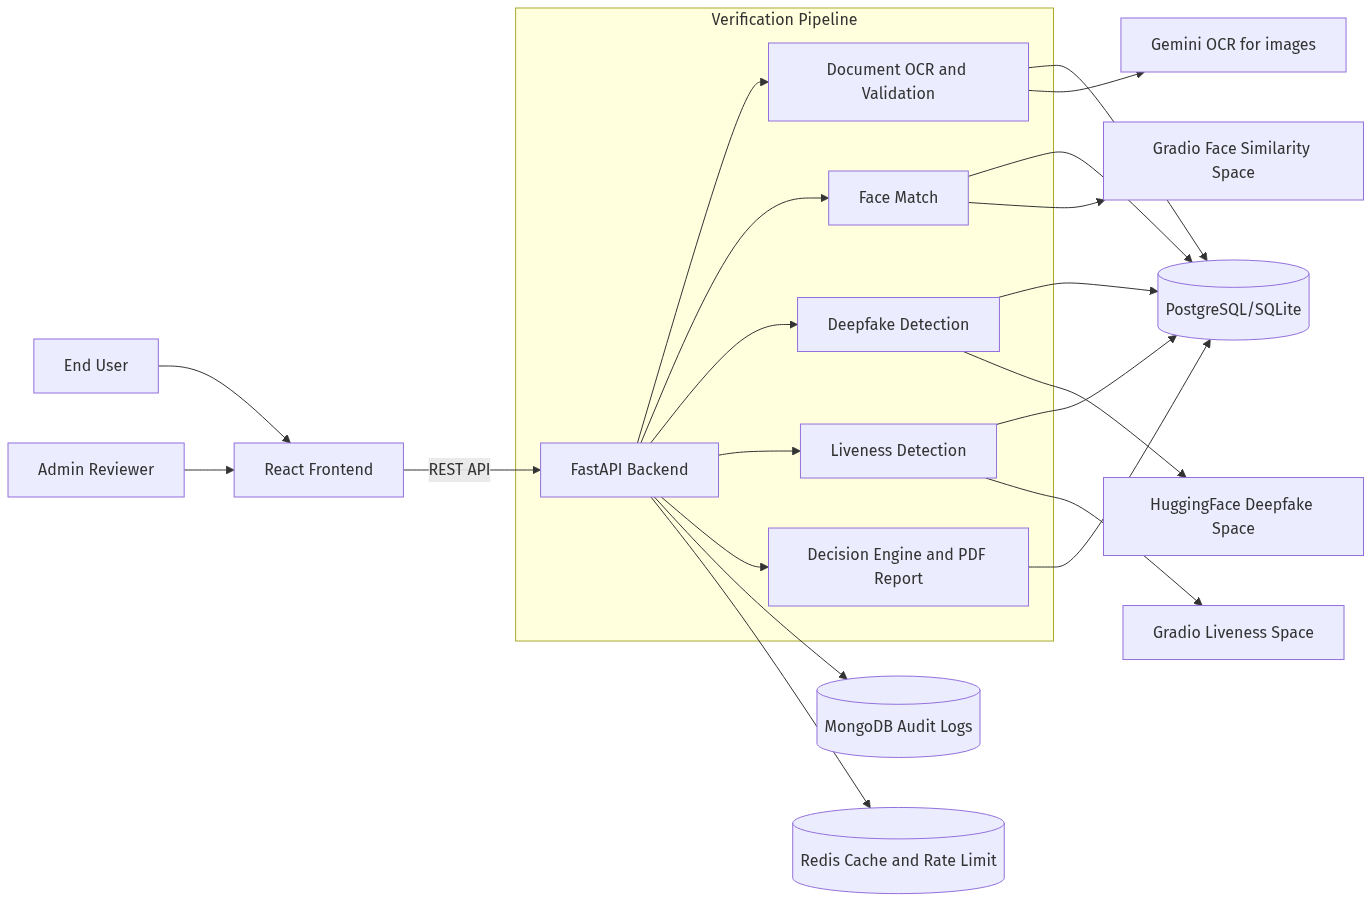
\includegraphics[width=\textwidth]{architecture_overview.png}
\caption{System Architecture Overview showing frontend, backend, databases, and external services}
\end{figure}

\begin{enumerate}
    \item \textbf{Stage 1 -- Document OCR:} User uploads an identity document. The backend sends the image to Google Gemini for structured field extraction, validates the results, extracts a face crop using dlib, and stores both the OCR data and image references.
    \item \textbf{Stage 2 -- Face Matching:} User provides a live selfie (file upload or webcam). The backend compares the document face crop against the selfie using an external face-similarity Gradio service and returns a percentage score.
    \item \textbf{Stage 3 -- Deepfake Detection:} The backend submits the selfie image to a HuggingFace-hosted AI image detector and returns a deepfake probability score.
    \item \textbf{Stage 4 -- Liveness Detection:} The backend submits the selfie to a Gradio-hosted liveness model and returns a liveness score.
    \item \textbf{Stage 5 -- Final Decision + Report:} An automated decision engine aggregates all four scores. If all thresholds are met, the session is approved; otherwise it is flagged for manual review. A PDF report is generated and downloadable.
\end{enumerate}

The administration layer provides a reviewer queue for flagged sessions and an analytics dashboard visible to admin and reviewer roles.

% =====================================================================
%  CHAPTER 3: PROJECT PLANNING AND SCHEDULING
% =====================================================================
\chapter{Project Planning and Scheduling}

\section{Work Breakdown Structure}

The project was decomposed into the following work packages:

\begin{table}[H]
\centering
\caption{Work Breakdown Structure}
\begin{tabular}{@{}clll@{}}
\toprule
\textbf{WBS ID} & \textbf{Work Package} & \textbf{Sub-Tasks} & \textbf{Deliverable} \\
\midrule
1.0 & Requirements & Literature review, SRS draft & SRS document \\
2.0 & Architecture & DB design, API design, module breakdown & Design doc \\
3.0 & Backend Core & Auth, DB models, migrations & Working API \\
4.0 & Document Module & Upload, OCR, validation, face extract & OCR endpoint \\
5.0 & Biometric Module & Face match, deepfake, liveness & 3 AI endpoints \\
6.0 & Decision + Report & Scoring engine, PDF generation & Report endpoint \\
7.0 & Admin Module & Review queue, decision API, analytics & Admin routes \\
8.0 & Frontend & Auth UI, 5 pipeline sections, dashboard & React app \\
9.0 & Integration & End-to-end pipeline testing & Working system \\
10.0 & Docker & Compose setup, environment config & docker-compose.yml \\
11.0 & Testing & Unit, integration, system tests & Test suite \\
12.0 & Documentation & Report, API docs, code comments & This report \\
\bottomrule
\end{tabular}
\end{table}

\section{Project Milestones}

\begin{table}[H]
\centering
\caption{Key Project Milestones}
\begin{tabular}{@{}clll@{}}
\toprule
\textbf{No.} & \textbf{Milestone} & \textbf{Target Week} & \textbf{Status} \\
\midrule
M1 & SRS approved & Week 3 & Completed \\
M2 & Database schema finalised & Week 5 & Completed \\
M3 & Auth module operational & Week 7 & Completed \\
M4 & Document OCR pipeline working & Week 10 & Completed \\
M5 & Face match + deepfake + liveness operational & Week 14 & Completed \\
M6 & Decision engine + PDF report working & Week 16 & Completed \\
M7 & Admin review queue working & Week 17 & Completed \\
M8 & Frontend all sections integrated & Week 20 & Completed \\
M9 & Analytics dashboard with charts & Week 21 & Completed \\
M10 & Docker Compose full stack working & Week 22 & Completed \\
M11 & All automated tests passing & Week 23 & Completed \\
M12 & Report submitted & Week 24 & Completed \\
\bottomrule
\end{tabular}
\end{table}

\section{Gantt Chart}

The project followed a 24-week schedule with overlapping phases to allow parallel development:

\begin{figure}[H]
\centering
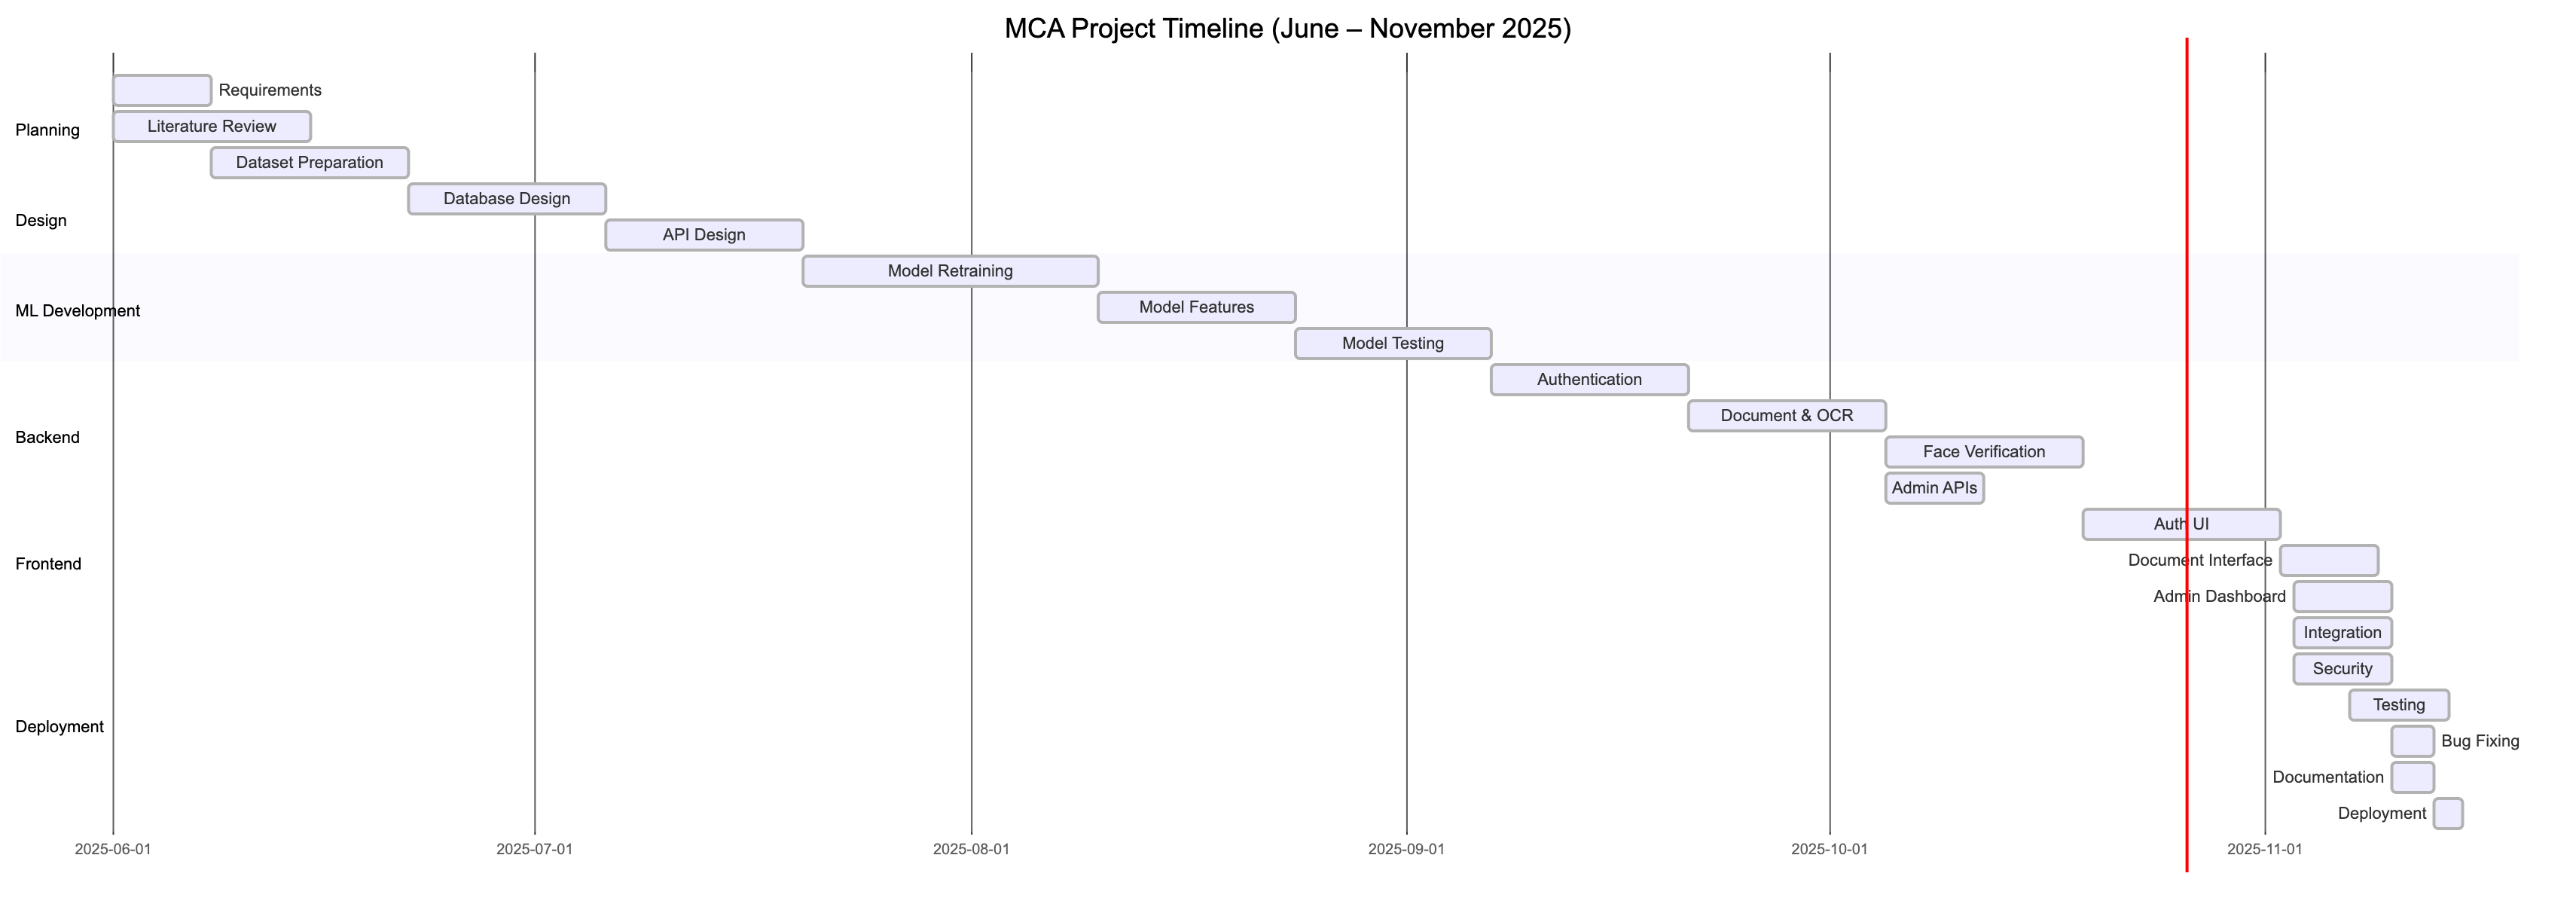
\includegraphics[width=\textwidth]{gantt_chart.png}
\caption{Gantt Chart showing the 24-week project timeline with overlapping phases}
\end{figure}

The overlapping design allowed backend and frontend development to proceed in parallel once the API contracts were established at Week 5, significantly reducing the overall project duration compared to a purely sequential waterfall approach.

\section{PERT Chart}

The Programme Evaluation and Review Technique (PERT) chart below shows the critical path through the project:

\begin{figure}[H]
\centering
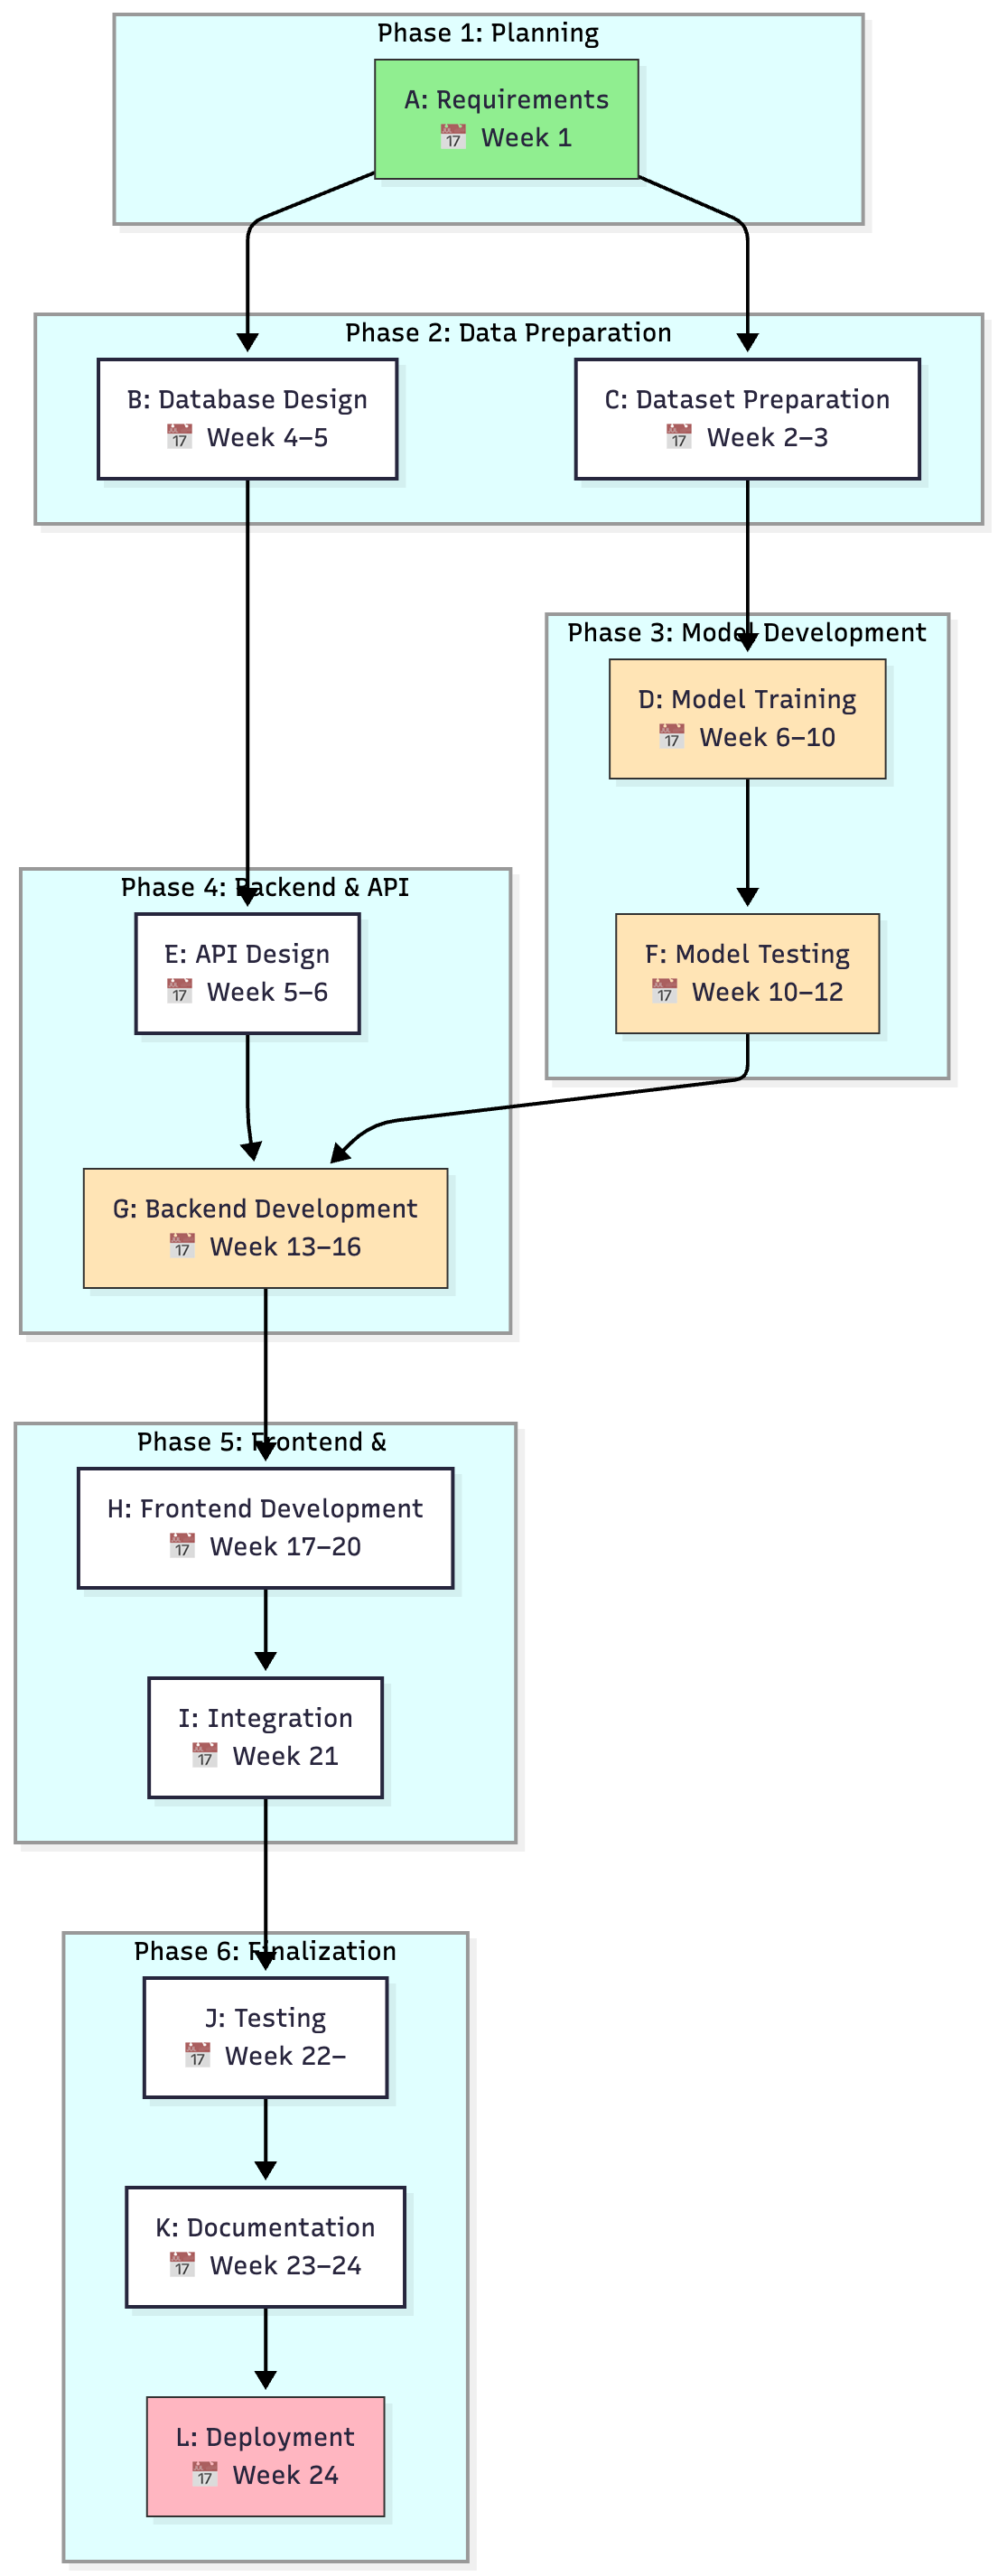
\includegraphics[width=0.8\textwidth]{pert_chart.png}
\caption{PERT Chart showing task dependencies and critical path}
\end{figure}

\textbf{Critical Path:}\\
Requirements Analysis $\rightarrow$ Database Design $\rightarrow$ Backend Core $\rightarrow$ Document OCR $\rightarrow$ Face Match $\rightarrow$ Deepfake Detection $\rightarrow$ Liveness $\rightarrow$ Decision Engine $\rightarrow$ PDF Report $\rightarrow$ Admin Module $\rightarrow$ Integration Testing $\rightarrow$ Submission

Total critical path duration: 24 weeks.

\section{Team Roles and Responsibilities}

\begin{table}[H]
\centering
\caption{Team Roles and Responsibilities}
\begin{tabular}{@{}lll@{}}
\toprule
\textbf{Role} & \textbf{Person} & \textbf{Responsibilities} \\
\midrule
Developer / Architect & Hardik Sharma & Full-stack implementation, all modules \\
Supervisor & Anshul Sharma & Technical review, guidance, approval \\
\bottomrule
\end{tabular}
\end{table}

\section{Risk Assessment and Mitigation}

\begin{table}[H]
\centering
\caption{Risk Register}
\begin{tabular}{@{}p{3.5cm}p{1.5cm}p{1.5cm}p{4.5cm}@{}}
\toprule
\textbf{Risk} & \textbf{Probability} & \textbf{Impact} & \textbf{Mitigation} \\
\midrule
External API unavailability (Gradio, HuggingFace) & Medium & High & Graceful error handling; mock responses for testing \\
Gemini OCR inaccuracy on low-quality documents & High & Medium & Pre-processing, quality scoring, user feedback \\
SQLite limitations in production & Low & Medium & Docker uses PostgreSQL; SQLite only for local dev \\
MongoDB unavailability & Low & Low & Audit logging degrades silently; app continues \\
JWT secret compromise & Low & Very High & Env var only; no hardcoding; documented in deployment notes \\
Scope creep & Medium & Medium & Strict in-scope/out-of-scope definition; deferred features listed \\
\bottomrule
\end{tabular}
\end{table}

\section{Timeline Deviations and Lessons Learned}

\begin{itemize}
    \item \textbf{OCR field extraction (Week 8-10):} Initial use of Tesseract OCR produced poor results on Indian identity documents due to varied fonts and layouts. This was replaced with Google Gemini 2.5 Flash Lite, which significantly improved extraction accuracy but required additional API integration work (+1 week).
    \item \textbf{dlib installation (Week 9):} Compiling dlib from source on macOS required resolving cmake and boost dependencies (+2 days).
    \item \textbf{Frontend webcam integration (Week 20):} Browser-based webcam capture using getUserMedia API required additional state management and a hidden canvas element for snapshot capture (+1 day).
    \item \textbf{Overall:} The project was delivered within the planned 24-week window, with no critical path delays.
\end{itemize}

% =====================================================================
%  CHAPTER 4: SOFTWARE REQUIREMENTS SPECIFICATION
% =====================================================================
\chapter{Software Requirements Specification}

\section{Introduction}

\subsection{Purpose}
This Software Requirements Specification (SRS) defines the complete functional and non-functional requirements for the AI-Based Real-Time eKYC System. It serves as the contractual agreement between the developer and the supervisor, and as the baseline against which the implemented system is validated.

\subsection{Document Conventions}
\begin{itemize}
    \item Requirements are tagged \textbf{FR-nn} (functional) or \textbf{NFR-nn} (non-functional).
    \item Priority is indicated as: \textbf{Must Have}, \textbf{Should Have}, or \textbf{Nice to Have}.
    \item Implementation status is: \textbf{Implemented}, \textbf{Partial}, or \textbf{Planned}.
\end{itemize}

\subsection{Intended Audience}
Developer, project supervisor, IGNOU evaluators.

\subsection{System Scope}
The system is a web-based eKYC platform consuming AI services for identity verification. It is not a government KYC system; it is an academic demonstration of an integrated AI pipeline for identity verification.

\section{Overall Description}

\subsection{Product Perspective}
The system is a standalone web application. It integrates with three categories of external services:
\begin{enumerate}
    \item \textbf{Google Generative AI} (Gemini 2.5 Flash Lite) for document OCR.
    \item \textbf{HuggingFace Inference API} for deepfake detection.
    \item \textbf{Gradio Spaces} for face similarity and liveness detection.
\end{enumerate}

\subsection{User Classes}

\begin{table}[H]
\centering
\caption{User Classes and Characteristics}
\begin{tabular}{@{}p{2.5cm}p{4cm}p{5cm}@{}}
\toprule
\textbf{User Class} & \textbf{Description} & \textbf{Primary Tasks} \\
\midrule
End User & General public seeking KYC verification & Register, upload document, provide selfie, view status, download report \\
Reviewer & Staff with KYC review authority & View flagged sessions, approve/reject/request re-upload \\
Admin & System administrator & All reviewer actions + view analytics, audit logs \\
\bottomrule
\end{tabular}
\end{table}

\subsection{Design and Implementation Constraints}
\begin{itemize}
    \item OCR accuracy depends on input document image quality.
    \item Face match and liveness scores depend on availability and performance of external Gradio-hosted models.
    \item Deepfake detection depends on HuggingFace Inference API availability.
    \item Local development uses SQLite; full production stack uses PostgreSQL.
    \item MongoDB and Redis are optional; the system degrades gracefully if unavailable.
\end{itemize}

\subsection{Assumptions and Dependencies}
\begin{itemize}
    \item Users have a device with a modern web browser (Chrome 90+, Firefox 88+, Safari 14+).
    \item Users have a camera for webcam-based selfie capture.
    \item \texttt{GEMINI\_API\_KEY}, \texttt{DEEPFAKE\_HF\_TOKEN}, \texttt{FACE\_SIMILARITY\_SPACE\_URL}, and \texttt{LIVENESS\_SPACE\_URL} are configured in the backend environment.
\end{itemize}

\section{Functional Requirements}

\begin{longtable}{@{}p{1.5cm}p{5cm}p{3cm}p{2.5cm}p{2.5cm}@{}}
\caption{Functional Requirements} \\
\toprule
\textbf{ID} & \textbf{Requirement} & \textbf{Priority} & \textbf{Status} & \textbf{Test ID} \\
\midrule
\endfirsthead
\multicolumn{5}{c}{\tablename\ \thetable{} -- continued} \\
\toprule
\textbf{ID} & \textbf{Requirement} & \textbf{Priority} & \textbf{Status} & \textbf{Test ID} \\
\midrule
\endhead
FR-01 & User registers with full\_name, email, phone, password; system validates uniqueness and returns JWT token & Must Have & Implemented & AUTH-01/02 \\
FR-02 & User logs in using email, phone, or full name plus password; system returns JWT token & Must Have & Implemented & AUTH-03/04 \\
FR-03 & Authenticated user can retrieve own profile (role, KYC status) via /auth/me & Must Have & Implemented & AUTH-05 \\
FR-04 & User can upload a document image (Aadhaar/PAN/Passport/DL/Voter ID) as JPEG, PNG, or PDF & Must Have & Implemented & DOC-01 \\
FR-05 & System extracts OCR fields (name, DOB, document number, address) using Gemini Vision API & Must Have & Implemented & DOC-04 \\
FR-06 & System validates document number format against type-specific regex patterns & Must Have & Implemented & DOC-04 \\
FR-07 & System calculates a document quality score and returns a recommendation & Should Have & Implemented & DOC-04 \\
FR-08 & System extracts and stores a face crop from the document image using dlib & Must Have & Implemented & DOC-04 \\
FR-09 & User provides a selfie image (file upload or webcam capture); system runs face similarity comparison & Must Have & Implemented & BIO-02 \\
FR-10 & Face match endpoint returns a percentage score and pass/fail result & Must Have & Implemented & BIO-02 \\
FR-11 & System screens the selfie through a deepfake detection model and returns a risk score & Must Have & Implemented & BIO-03 \\
FR-12 & System runs liveness detection on the selfie and returns a liveness score & Must Have & Implemented & BIO-04 \\
FR-13 & Decision engine aggregates all four scores and determines approved or manual\_review & Must Have & Implemented & DEC-03 \\
FR-14 & System generates a downloadable PDF verification report after final decision & Must Have & Implemented & DEC-03 \\
FR-15 & Reviewer/admin can list all flagged (manual\_review) sessions & Must Have & Implemented & ADM-01 \\
FR-16 & Reviewer/admin can approve, reject, or request re-upload for a flagged session & Must Have & Implemented & ADM-04 \\
FR-17 & Rejection requires a reason string; system enforces this at the API level & Must Have & Implemented & ADM-03 \\
FR-18 & Admin can view analytics overview (total users, sessions, approvals, rejections, flagged) & Should Have & Implemented & ANA-01 \\
FR-19 & Admin can view 30-day daily trend data (approved/rejected/flagged per day) & Should Have & Implemented & ANA-02 \\
FR-20 & Admin can view per-stage average and P95 latency data & Should Have & Implemented & ANA-03 \\
FR-21 & System writes audit log entries to MongoDB for auth and review events & Should Have & Partial & AUD-01 \\
FR-22 & Authenticated image requests are proxied through a protected endpoint requiring a valid JWT & Must Have & Implemented & SEC-04 \\
\bottomrule
\end{longtable}

\section{Non-Functional Requirements}

\subsection{Performance Requirements (NFR-01)}
\begin{itemize}
    \item API response time for all non-AI endpoints (auth, session CRUD, analytics): $<$500~ms at p95 under normal load.
    \item Document OCR stage: dependent on Gemini API; typically 3--10~s.
    \item Face match stage: dependent on Gradio Space; typically 2--5~s.
    \item Deepfake detection: dependent on HuggingFace Inference API; typically 5--15~s.
    \item Liveness detection: dependent on Gradio Space; typically 2--5~s.
    \item PDF generation: $<$2~s for a typical report payload.
\end{itemize}

\subsection{Security Requirements (NFR-02)}
\begin{itemize}
    \item All passwords stored as bcrypt hash with cost factor 12.
    \item JWT tokens signed with HS256; configurable expiry (default 24~h).
    \item All API routes requiring authentication return HTTP 401 if no valid token is presented.
    \item Admin and reviewer routes return HTTP 403 if the token holder's role is insufficient.
    \item File uploads are validated for MIME type, extension, and size before processing.
    \item Rate limiting applied to all auth routes using slowapi.
    \item Input strings are sanitised before storage.
\end{itemize}

\subsection{Reliability Requirements (NFR-03)}
\begin{itemize}
    \item Application startup creates all required database tables automatically (\texttt{AUTO\_CREATE\_SCHEMA=true}).
    \item External service failures (Gradio, HuggingFace, MongoDB, Redis) are caught and mapped to appropriate HTTP error responses; the core application remains operational.
    \item A \texttt{/api/v1/system/health} endpoint returns the status of all dependent services.
\end{itemize}

\subsection{Maintainability Requirements (NFR-04)}
\begin{itemize}
    \item Backend follows a layered architecture: \texttt{api/routes} $\rightarrow$ \texttt{services} $\rightarrow$ \texttt{models} $\leftrightarrow$ \texttt{db/session}.
    \item Frontend components are TypeScript-typed with explicit prop interfaces.
    \item All API endpoints are documented via FastAPI's auto-generated OpenAPI schema.
    \item Database schema changes are managed via Alembic migrations.
\end{itemize}

\subsection{Portability Requirements (NFR-05)}
\begin{itemize}
    \item The full stack can be started with a single \texttt{docker compose up -d --build} command.
    \item Local development (without Docker) requires only Python 3.12, Node.js 18+, and environment variable configuration.
    \item The system supports both SQLite (local) and PostgreSQL (Docker/production) without code changes.
\end{itemize}

\subsection{Scalability Requirements (NFR-06)}
\begin{itemize}
    \item FastAPI's async architecture enables handling multiple concurrent requests without thread blocking.
    \item Redis is integrated as a rate-limit store and cache, allowing horizontal scaling of backend instances.
    \item PostgreSQL supports connection pooling and read replicas for production scale-out.
\end{itemize}

\section{External Interface Requirements}

\subsection{User Interface}
\begin{itemize}
    \item Single-page web application accessible via standard desktop and tablet browsers.
    \item Responsive layout with a sticky header, 5-step pipeline progress indicator, and section-based scrollable content.
    \item Toast notifications for all operations (success, warning, error).
    \item Collapsible raw JSON output for debugging.
\end{itemize}

\subsection{Hardware Interface}
\begin{itemize}
    \item Server: any x86\_64 machine with 4+ GB RAM and Python 3.12.
    \item Client: any device with a modern browser and an optional camera for webcam selfie capture.
\end{itemize}

\subsection{Software Interfaces}
\begin{table}[H]
\centering
\caption{External Software Interfaces}
\begin{tabular}{@{}llll@{}}
\toprule
\textbf{System} & \textbf{Protocol} & \textbf{Config Var} & \textbf{Purpose} \\
\midrule
Google Gemini API & HTTPS / REST & GEMINI\_API\_KEY & Document OCR \\
HuggingFace Inference & HTTPS / REST & DEEPFAKE\_HF\_TOKEN & Deepfake scoring \\
Gradio Face Similarity & HTTPS / SSE & FACE\_SIMILARITY\_SPACE\_URL & Face matching \\
Gradio Liveness & HTTPS / SSE & LIVENESS\_SPACE\_URL & Liveness scoring \\
PostgreSQL / SQLite & TCP / file & DATABASE\_URL & Persistent data \\
MongoDB & TCP & MONGODB\_URI & Audit logs \\
Redis & TCP & REDIS\_URL & Rate limiting, cache \\
\bottomrule
\end{tabular}
\end{table}

\section{Acceptance Criteria}

The following acceptance criteria define the minimum viable delivered system:

\begin{enumerate}
    \item A new user can register, login, and receive a JWT token. (\textit{AUTH-01})
    \item A user can upload a PAN/Aadhaar document and receive OCR-extracted fields. (\textit{DOC-04})
    \item A user can submit a selfie and receive a face match score. (\textit{BIO-02})
    \item A user can receive deepfake and liveness scores for a submitted selfie. (\textit{BIO-03, BIO-04})
    \item A user can generate and download a PDF report after completing all pipeline stages. (\textit{DEC-03})
    \item An admin can view the flagged session queue and approve a session. (\textit{ADM-04})
    \item Analytics endpoints return valid aggregate data for admin tokens. (\textit{ANA-01})
    \item All 11 backend tests and 10 frontend tests pass. (\textit{Automated test suite})
\end{enumerate}

% =====================================================================
%  CHAPTER 5: ENGINEERING PARADIGM AND METHODOLOGY
% =====================================================================
\chapter{Engineering Paradigm and Methodology}

\section{SDLC Approach}

\subsection{Iterative and Incremental Development}

The project followed an \textbf{iterative and incremental} approach inspired by Agile principles, rather than a strict waterfall model. This choice was motivated by:

\begin{itemize}
    \item \textbf{Evolving requirements:} The exact API contracts for external services (Gradio, HuggingFace) were discovered during implementation and required iterative adjustment.
    \item \textbf{Tight feedback loop:} Working software was available after each stage of the pipeline was implemented, allowing early validation.
    \item \textbf{Risk mitigation:} High-risk components (external AI services) were prototyped and integrated early, reducing late-stage surprises.
\end{itemize}

Development was organised into 2-week sprints, each with a specific deliverable:

\begin{table}[H]
\centering
\caption{Sprint Plan}
\begin{tabular}{@{}clll@{}}
\toprule
\textbf{Sprint} & \textbf{Weeks} & \textbf{Focus} & \textbf{Deliverable} \\
\midrule
1 & 1--2 & Requirements, architecture & SRS, DB schema \\
2 & 3--4 & Backend core & Auth, DB models, health endpoint \\
3 & 5--6 & Document module & Upload + OCR endpoint \\
4 & 7--8 & Face extraction & dlib integration, face crop storage \\
5 & 9--10 & Face match + deepfake & Gradio + HuggingFace integration \\
6 & 11--12 & Liveness + decision & Liveness endpoint + scoring engine \\
7 & 13--14 & PDF report & WeasyPrint generation + download \\
8 & 15--16 & Admin module & Review queue + analytics endpoints \\
9 & 17--18 & Frontend core & Auth UI + OCR + face match sections \\
10 & 19--20 & Frontend pipeline & Deepfake, liveness, report sections \\
11 & 21--22 & Frontend analytics + Docker & Chart.js dashboard + Compose setup \\
12 & 23--24 & Testing + documentation & All tests passing, report written \\
\bottomrule
\end{tabular}
\end{table}

\section{Modular Architecture Philosophy}

The system follows a \textbf{separation of concerns} principle with clearly defined module boundaries:

\begin{enumerate}
    \item \textbf{Authentication Module:} Handles all identity-related concerns -- registration, login, JWT issuance, token validation, and role resolution. No business logic from other modules bleeds into this layer.
    \item \textbf{Feature Pipeline Module:} Implements the five-stage verification pipeline as a single coherent route group (\texttt{/api/v1/features/}). Each stage builds on the previous one through in-memory session state.
    \item \textbf{Admin Module:} Provides review queue and decision APIs restricted to reviewer/admin roles. Decoupled from the feature pipeline.
    \item \textbf{Analytics Module:} Provides aggregation queries over verification sessions. Read-only; does not mutate any data.
    \item \textbf{Audit Module:} Writes to MongoDB. Implemented as a fire-and-forget async call that never blocks the main request flow.
    \item \textbf{Frontend Components:} React components are organised by function (auth, pipeline stages, dashboard, layout, shared). Each component receives data through typed props and calls API functions from the centralised \texttt{services/api.ts} module.
\end{enumerate}

\section{API-First Design}

The backend was designed API-first: the OpenAPI schema was defined before frontend development began, ensuring a stable contract between the two layers. FastAPI auto-generates and serves this schema at \texttt{/docs} (Swagger UI) and \texttt{/redoc} (ReDoc).

All API functions on the frontend return a typed \texttt{\{data, error\}} object, isolating error handling from business logic.

\section{Test-Driven Mindset}

While the project did not follow strict Test-Driven Development (TDD), tests were written alongside implementation rather than after, particularly for:
\begin{itemize}
    \item Auth routes (register, login, profile) -- verifying security boundaries.
    \item Frontend components (LoginForm, ScoreCard, Toast) -- verifying rendering and interaction.
\end{itemize}

\section{Traceability Matrix}

\begin{table}[H]
\centering
\caption{Requirements Traceability Matrix (Sample)}
\begin{tabular}{@{}llll@{}}
\toprule
\textbf{FR ID} & \textbf{Module} & \textbf{File} & \textbf{Test ID} \\
\midrule
FR-01 & Auth & \texttt{app/api/routes/auth.py} & AUTH-01 \\
FR-02 & Auth & \texttt{app/api/routes/auth.py} & AUTH-03 \\
FR-05 & Document & \texttt{app/services/document\_processing.py} & DOC-04 \\
FR-08 & Document & \texttt{app/services/document\_face\_extraction.py} & DOC-04 \\
FR-09 & Feature & \texttt{app/api/routes/features.py} & BIO-02 \\
FR-11 & Feature & \texttt{app/services/deepfake\_inference.py} & BIO-03 \\
FR-13 & Feature & \texttt{app/api/routes/features.py} & DEC-03 \\
FR-18 & Analytics & \texttt{app/api/routes/analytics.py} & ANA-01 \\
\bottomrule
\end{tabular}
\end{table}

% =====================================================================
%  CHAPTER 6: SYSTEM MODELING AND DIAGRAMS
% =====================================================================
\chapter{System Modeling and Diagrams}

\section{Data Flow Diagrams}

\subsection{DFD Level 0 -- Context Diagram}

The Level 0 DFD (Context Diagram) shows the eKYC system as a single process interacting with three external entities:

\begin{figure}[H]
\centering
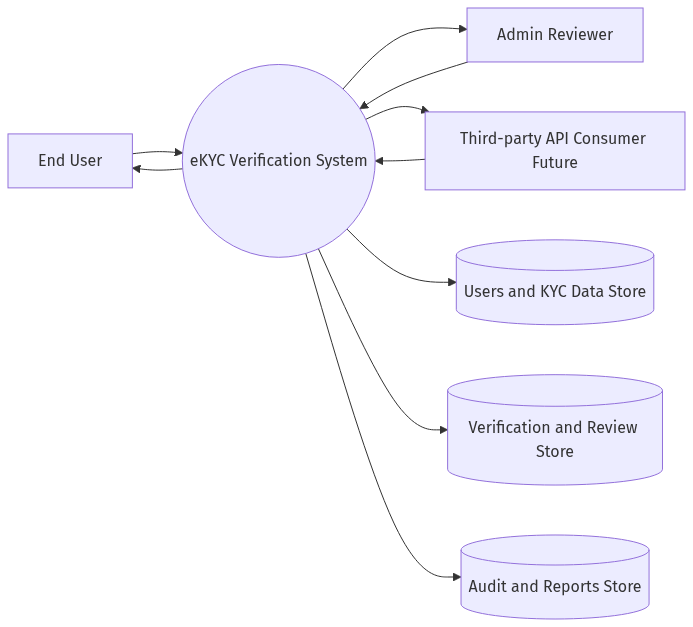
\includegraphics[width=0.8\textwidth]{dfd_level0.png}
\caption{DFD Level 0 -- System Context Diagram}
\end{figure}

\textbf{External Entities:}
\begin{itemize}
    \item \textbf{End User:} Provides personal information, identity documents, and selfie images. Receives KYC status and PDF report.
    \item \textbf{Admin/Reviewer:} Receives flagged session data. Provides review decisions.
    \item \textbf{AI Services:} External platforms (Gemini, HuggingFace, Gradio) that receive document/image data and return analysis results.
\end{itemize}

\subsection{DFD Level 1}

The Level 1 DFD decomposes the system into seven major processes:

\begin{figure}[H]
\centering
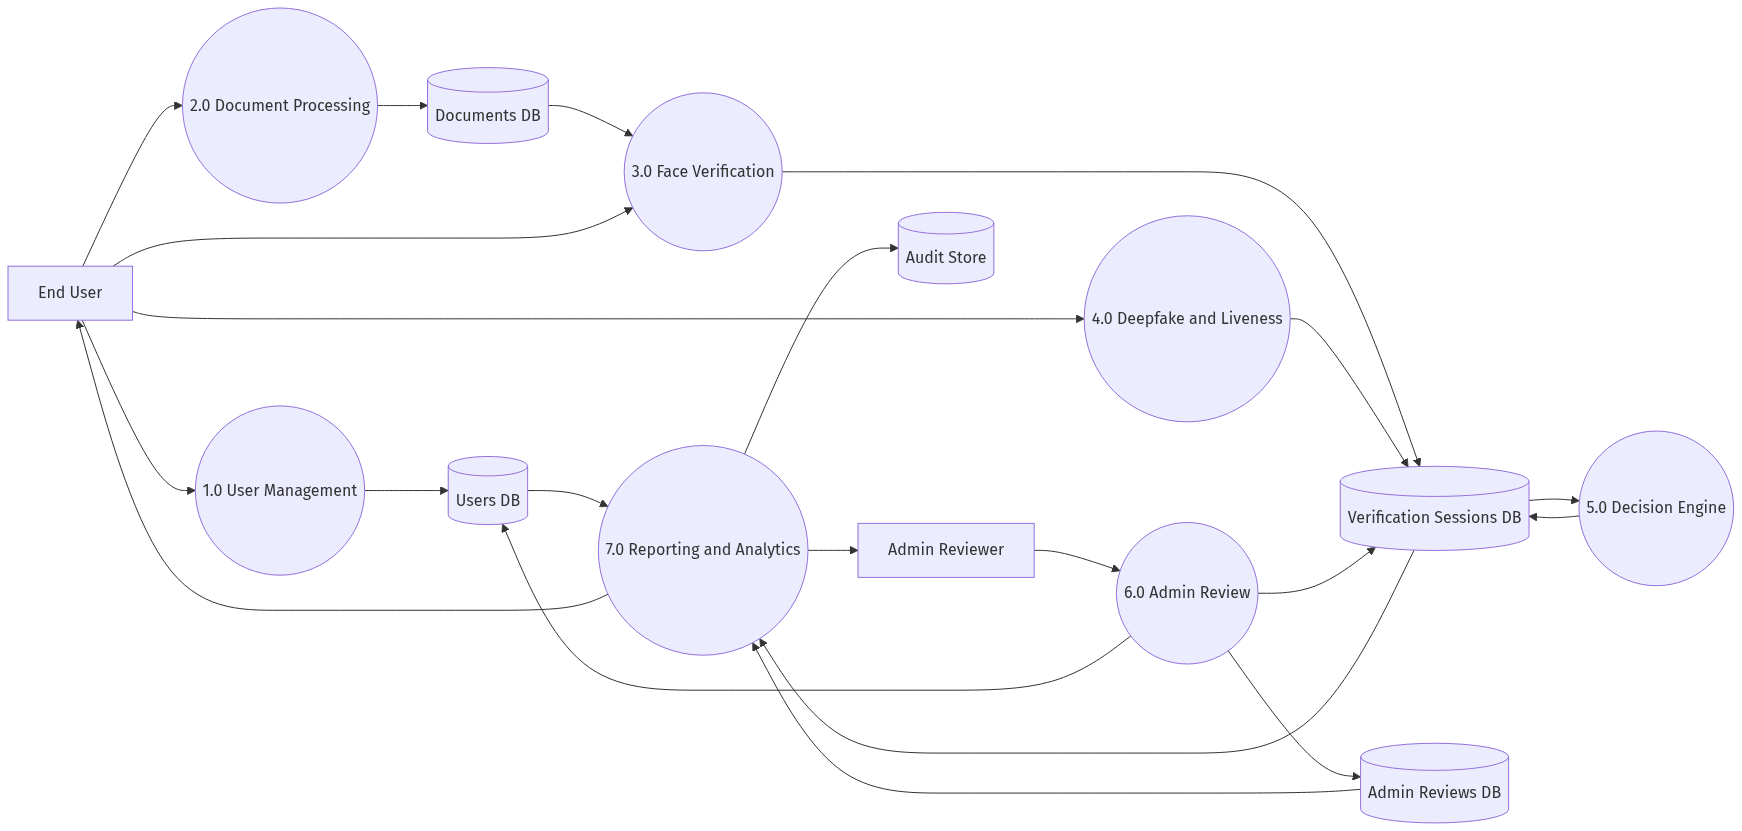
\includegraphics[width=\textwidth]{dfd_level1.png}
\caption{DFD Level 1 -- Major System Processes}
\end{figure}

\textbf{Process Descriptions:}

\textbf{1.0 -- User Management:} Handles registration, login, and profile management. Reads/writes the Users data store. Outputs JWT tokens to authenticated entities.

\textbf{2.0 -- Document Processing:} Receives document images from the End User. Sends them to the OCR Engine (Gemini). Validates extracted data and invokes face extraction. Writes to the Documents data store.

\textbf{3.0 -- Face Verification:} Receives the reference face crop (from Process 2.0) and the live selfie image. Invokes the Gradio face-similarity service. Writes match score and image references to the Sessions data store.

\textbf{4.0 -- Deepfake \& Liveness Detection:} Receives the live selfie image. Invokes the HuggingFace deepfake model and the Gradio liveness model. Writes scores to the Sessions data store.

\textbf{5.0 -- Decision Engine:} Reads all scores from the Sessions data store. Applies thresholds. Writes the final KYC decision to both the Sessions and Users data stores.

\textbf{6.0 -- Admin Review:} Reads flagged sessions from the Sessions data store. Presents them to the Admin/Reviewer entity. Receives review decisions and updates the Reviews and Sessions data stores.

\textbf{7.0 -- Reporting:} Reads session data and generates PDF reports. Writes to the Audit Logs data store. Provides reports to the End User and analytics data to the Admin.

\section{Use Case Diagram}

\begin{figure}[H]
\centering
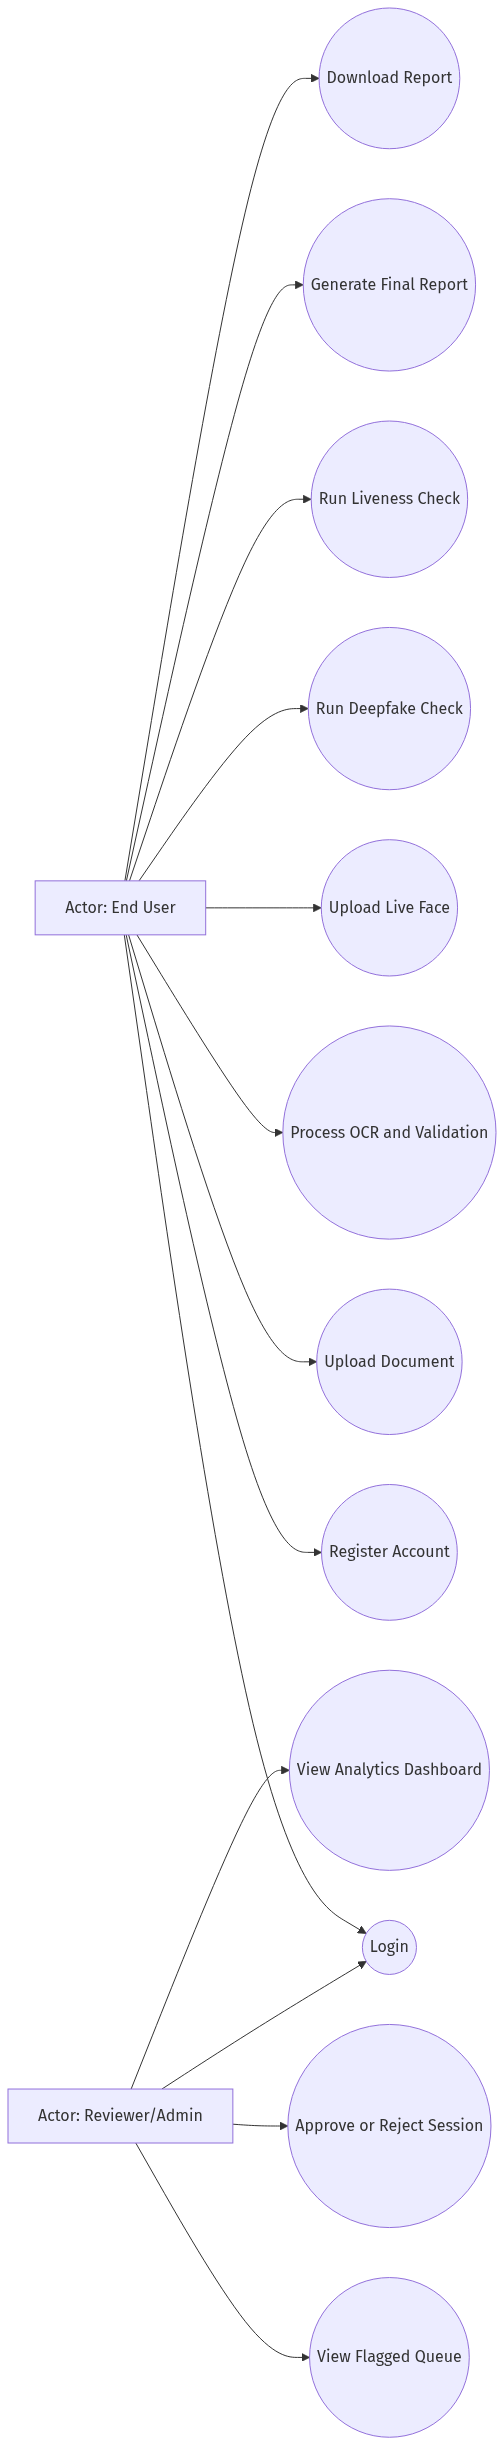
\includegraphics[width=\textwidth]{use_case_diagram.png}
\caption{Use Case Diagram showing actor-system interactions}
\end{figure}

\textbf{Actor: End User}
\begin{itemize}
    \item UC-01: Register Account
    \item UC-02: Login
    \item UC-03: Upload Identity Document
    \item UC-04: Provide Selfie (Upload or Webcam)
    \item UC-05: View Verification Status
    \item UC-06: Download PDF Report
    \item UC-07: Logout
\end{itemize}

\textbf{Actor: Reviewer (extends End User)}
\begin{itemize}
    \item UC-08: View Flagged Session Queue
    \item UC-09: Approve Flagged Session
    \item UC-10: Reject Flagged Session
    \item UC-11: Request Document Re-Upload
\end{itemize}

\textbf{Actor: Admin (extends Reviewer)}
\begin{itemize}
    \item UC-12: View Analytics Dashboard
    \item UC-13: View Audit Logs
    \item UC-14: Manage Users
\end{itemize}

\section{Activity Diagram -- Verification Workflow}

\begin{figure}[H]
\centering
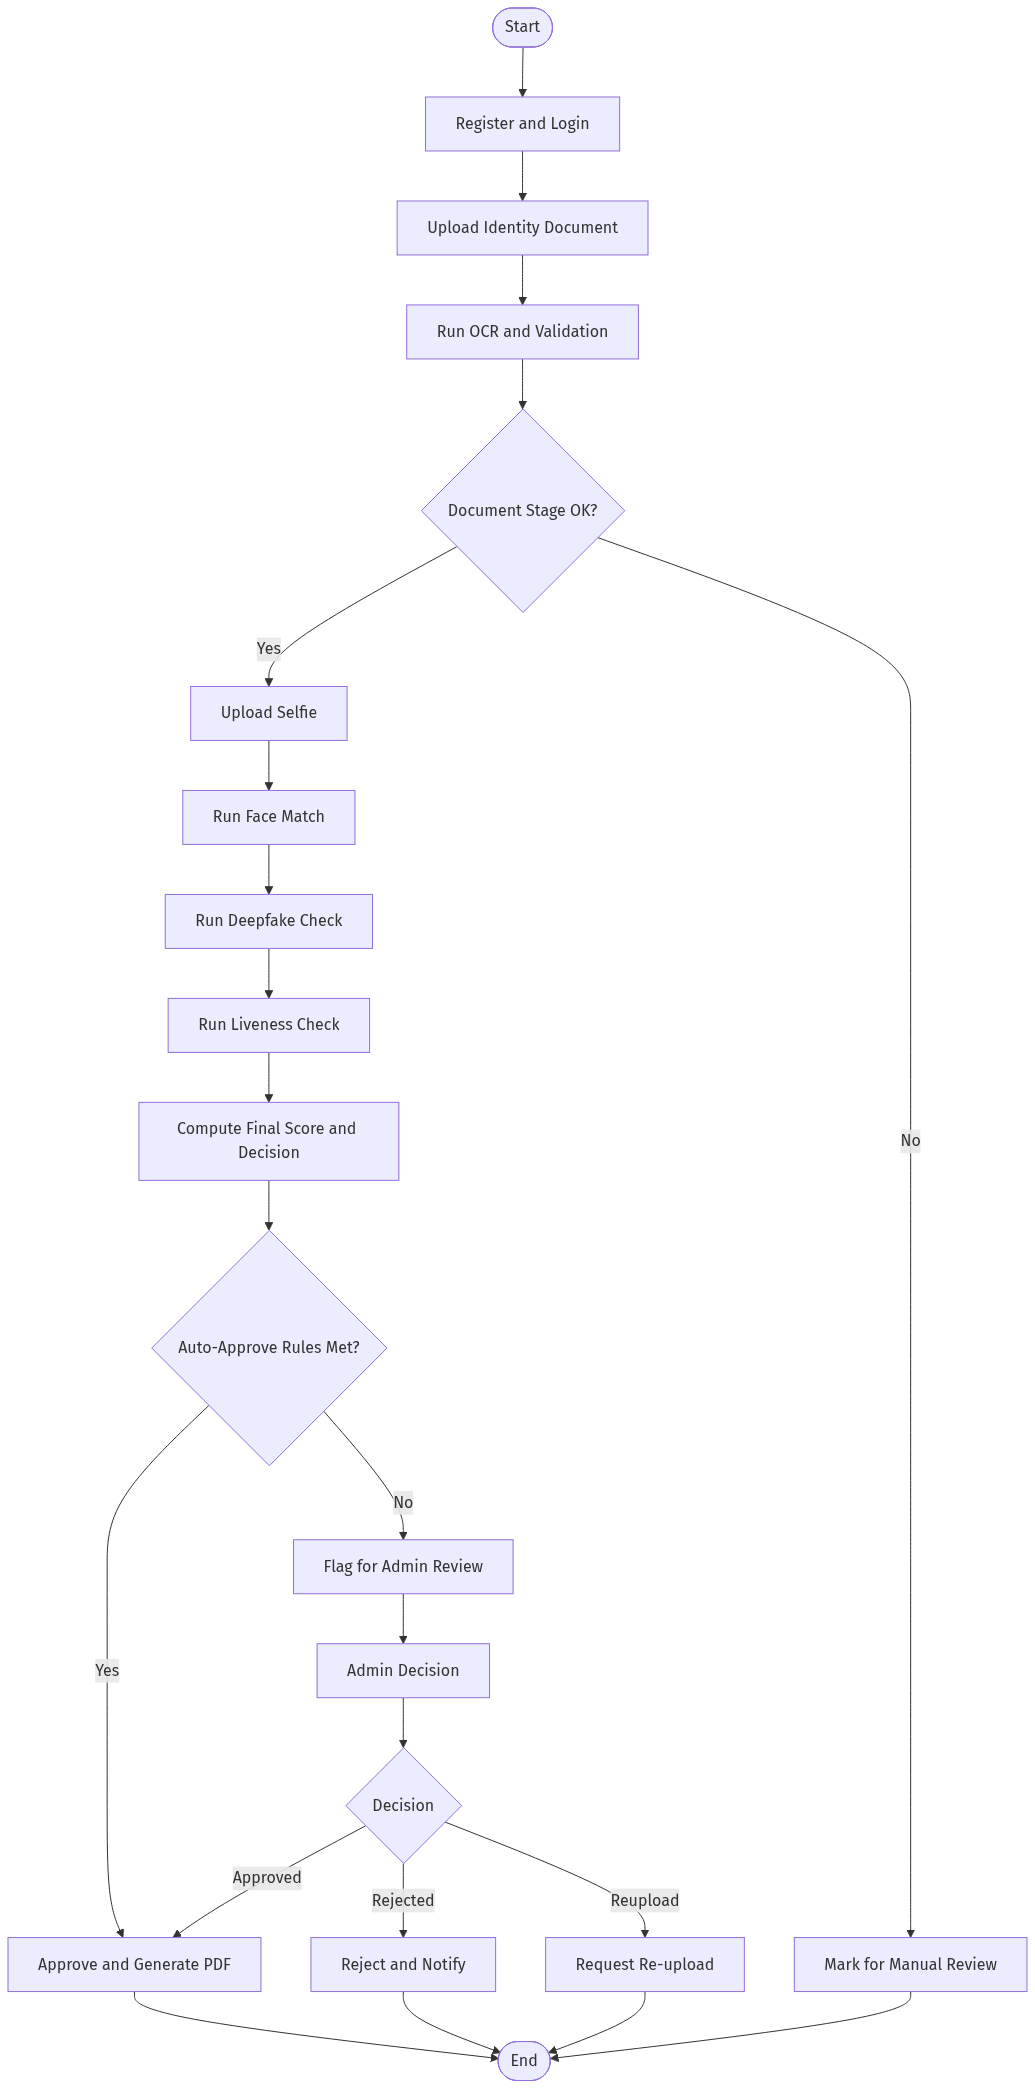
\includegraphics[width=\textwidth]{activity_workflow.png}
\caption{Activity Diagram showing the full user verification workflow}
\end{figure}

The verification workflow proceeds as follows:
\begin{enumerate}
    \item User registers and logs in.
    \item User uploads an identity document. System performs OCR extraction and face crop.
    \item If OCR fails quality checks, user is prompted to re-upload.
    \item User provides a live selfie (upload or webcam).
    \item System runs face match, deepfake detection, and liveness in parallel.
    \item Decision engine evaluates all scores.
    \item \textbf{Branch A (All thresholds met):} Session is automatically approved. PDF report generated. User notified.
    \item \textbf{Branch B (Any threshold failed):} Session flagged for manual review.
    \item Admin reviews flagged session: approves, rejects, or requests re-upload.
    \item User is notified of the final decision.
\end{enumerate}

\section{Sequence Diagrams}

\subsection{User Verification Sequence}

\begin{figure}[H]
\centering
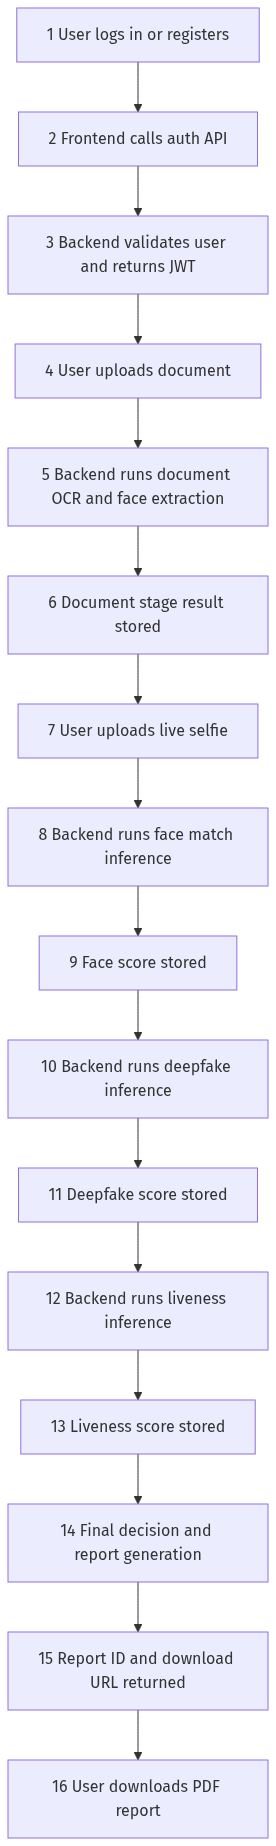
\includegraphics[width=\textwidth]{sequence_user_verification.png}
\caption{Sequence Diagram -- User Identity Verification Flow}
\end{figure}

The sequence shows interactions between: Browser, React SPA, FastAPI Backend, Gemini API, Gradio Face Service, HuggingFace API, and PostgreSQL Database.

Key interaction steps:
\begin{enumerate}
    \item User POSTs credentials $\rightarrow$ Backend validates $\rightarrow$ Returns JWT.
    \item User POSTs document image $\rightarrow$ Backend calls Gemini $\rightarrow$ Returns OCR data + face crop URL.
    \item User POSTs selfie $\rightarrow$ Backend calls Gradio face-similarity $\rightarrow$ Returns match score.
    \item Backend calls HuggingFace deepfake model $\rightarrow$ Returns deepfake probability.
    \item Backend calls Gradio liveness model $\rightarrow$ Returns liveness score.
    \item Backend runs decision engine $\rightarrow$ Persists decision $\rightarrow$ Returns final report.
\end{enumerate}

\subsection{Admin Review Sequence}

\begin{figure}[H]
\centering
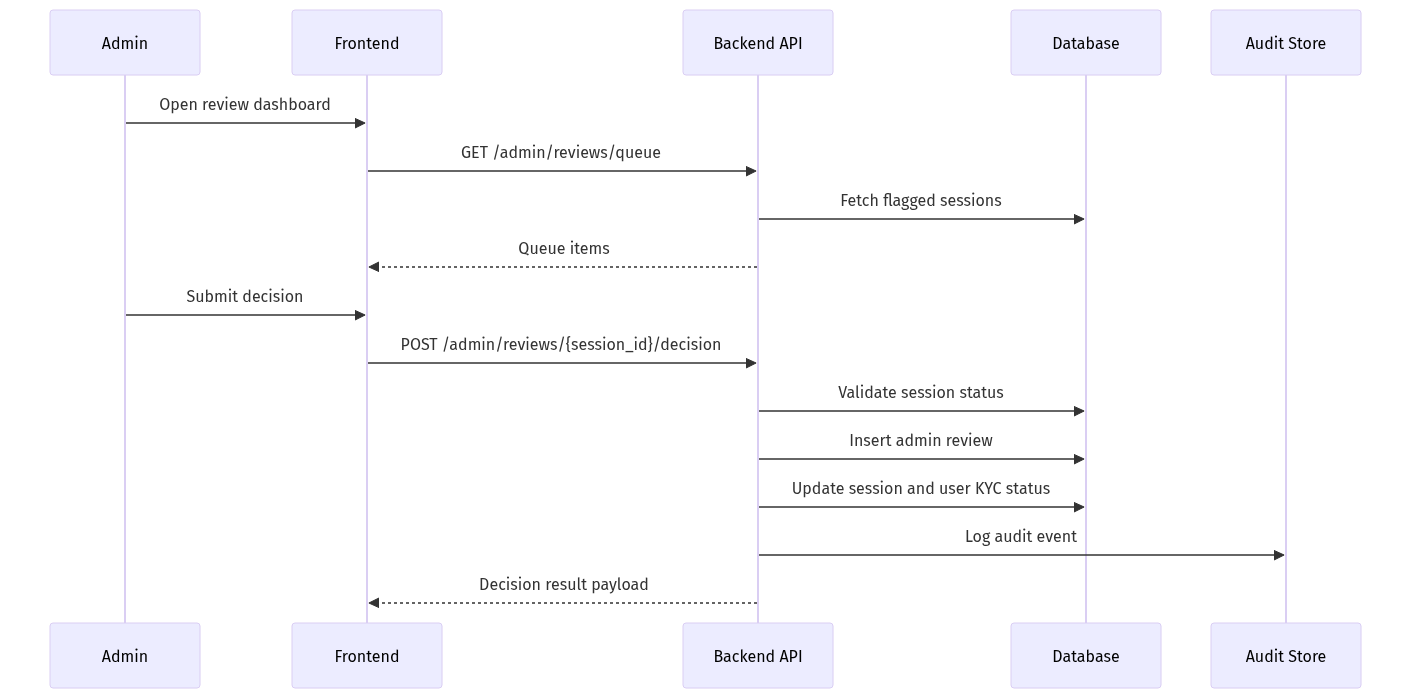
\includegraphics[width=\textwidth]{sequence_admin_review.png}
\caption{Sequence Diagram -- Admin Review Workflow}
\end{figure}

\section{State Machine Diagram -- Verification Session}

\begin{figure}[H]
\centering
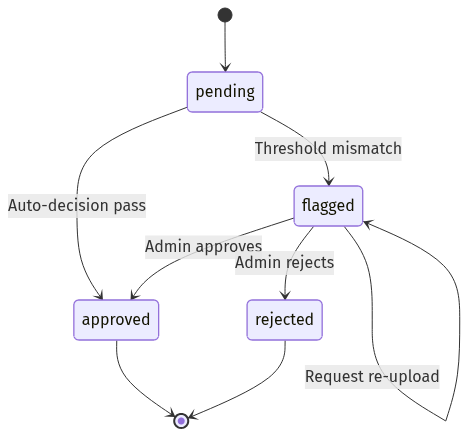
\includegraphics[width=0.75\textwidth]{state_verification_session.png}
\caption{State Machine Diagram for a Verification Session}
\end{figure}

\textbf{States:}
\begin{itemize}
    \item \textbf{pending:} Initial state when a session is created.
    \item \textbf{approved:} All AI scores meet thresholds; auto-approved by decision engine.
    \item \textbf{flagged:} One or more scores fail thresholds; awaiting manual review.
    \item \textbf{rejected:} Admin explicitly rejected the session.
\end{itemize}

\textbf{Transitions:}
\begin{itemize}
    \item pending $\rightarrow$ approved: all thresholds met after final report generation.
    \item pending $\rightarrow$ flagged: any threshold failed.
    \item flagged $\rightarrow$ approved: admin approves.
    \item flagged $\rightarrow$ rejected: admin rejects.
    \item flagged $\rightarrow$ pending: admin requests re-upload (user must restart pipeline).
\end{itemize}

\section{Class Diagram -- Backend Domain Model}

\begin{figure}[H]
\centering
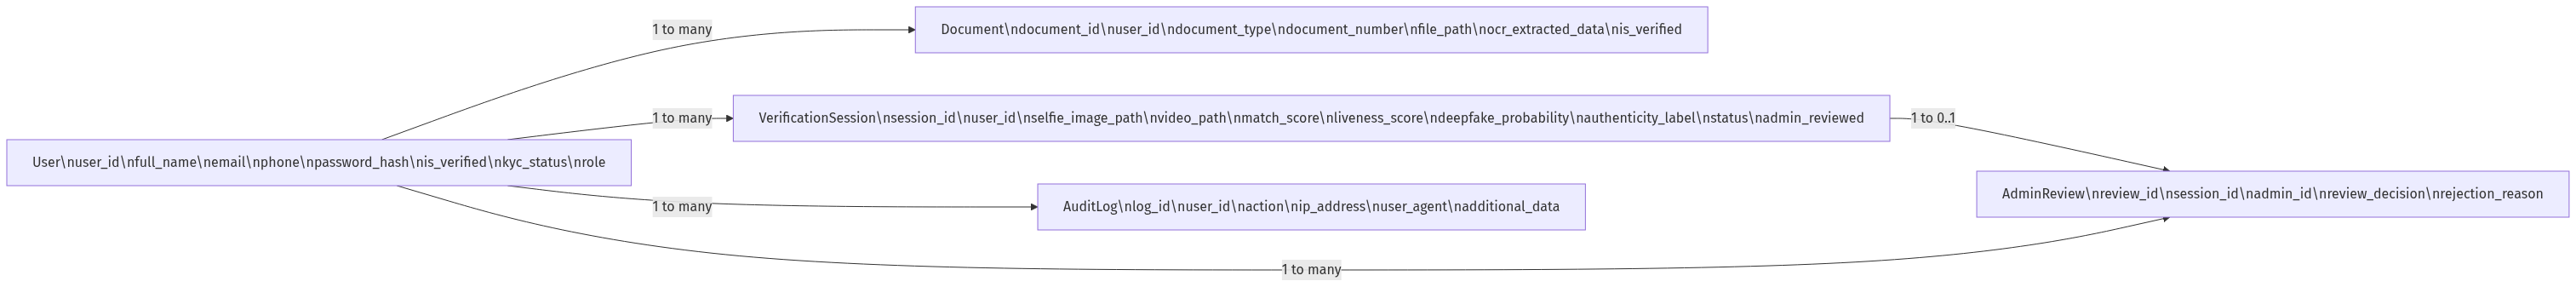
\includegraphics[width=\textwidth]{class_backend_domain.png}
\caption{Class Diagram -- Backend Domain Model}
\end{figure}

The backend domain model consists of five primary entities:

\begin{itemize}
    \item \textbf{User} -- Central entity with role (user/admin/reviewer) and KYC status. One-to-many relationships with Document, VerificationSession, and AuditLog.
    \item \textbf{Document} -- Represents an uploaded identity document with OCR-extracted data stored as JSON.
    \item \textbf{VerificationSession} -- Stores all pipeline scores, image paths, and the final decision. One-to-one relationship with AdminReview.
    \item \textbf{AdminReview} -- Records the reviewer's decision for a flagged session.
    \item \textbf{AuditLog} -- Records timestamped actions for compliance purposes (stored in MongoDB).
\end{itemize}

\section{ER Diagram}

\begin{figure}[H]
\centering
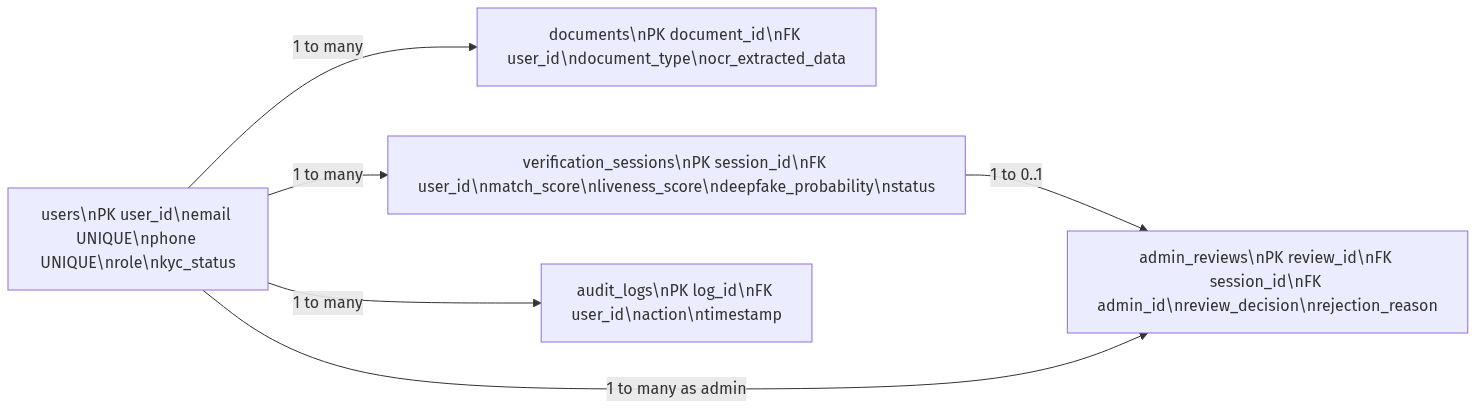
\includegraphics[width=\textwidth]{er_database.png}
\caption{Entity-Relationship Diagram}
\end{figure}

\textbf{Relationships and Cardinalities:}
\begin{itemize}
    \item \textbf{USER -- DOCUMENT:} 1:N (one user can upload many documents; cascade delete).
    \item \textbf{USER -- VERIFICATION\_SESSION:} 1:N (one user can have multiple sessions; cascade delete).
    \item \textbf{VERIFICATION\_SESSION -- ADMIN\_REVIEW:} 1:1 (each flagged session has at most one review).
    \item \textbf{USER (admin) -- ADMIN\_REVIEW:} 1:N (one admin can review many sessions; set null on admin deletion).
    \item \textbf{USER -- AUDIT\_LOG:} 1:N (each action generates a log entry; set null if user deleted).
\end{itemize}

\section{Deployment Diagram}

\begin{figure}[H]
\centering
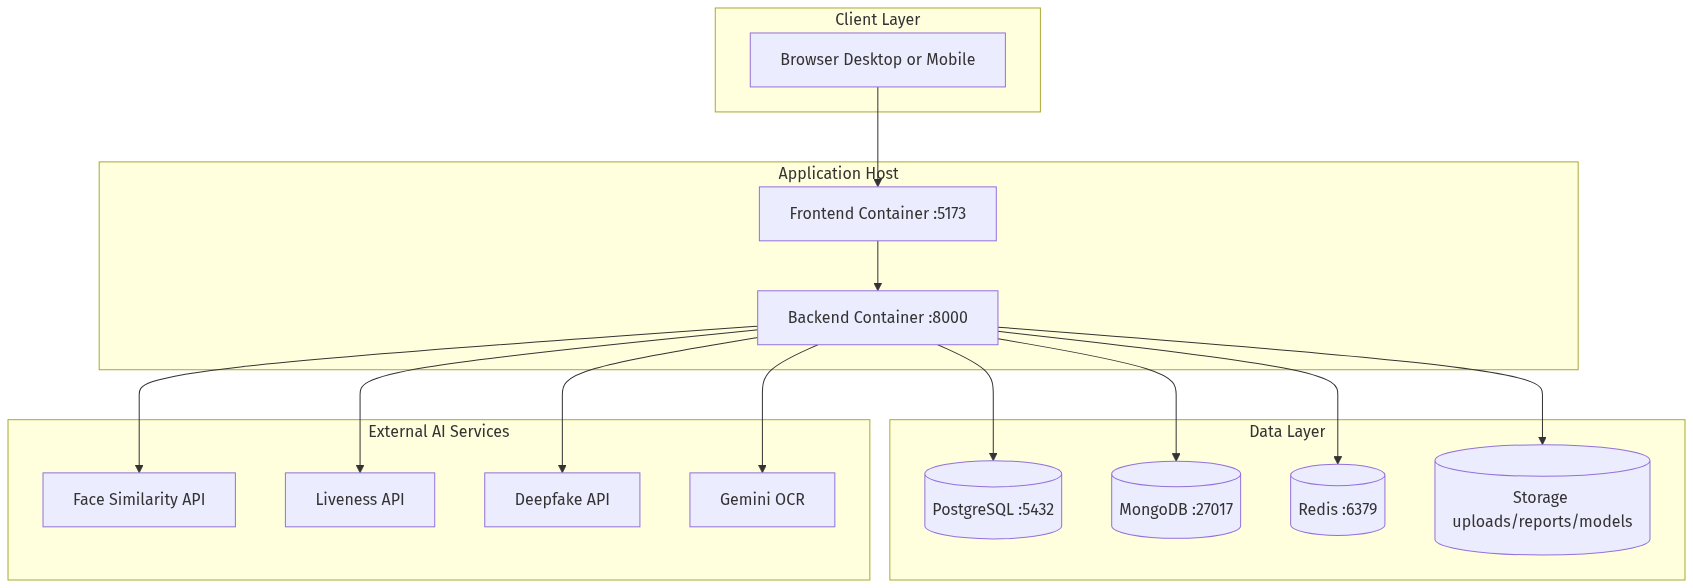
\includegraphics[width=\textwidth]{deployment_diagram.png}
\caption{Deployment Diagram showing Docker Compose service topology}
\end{figure}

The Docker Compose deployment topology:
\begin{itemize}
    \item \textbf{frontend} container: Nginx serving the React SPA on port 80/443; communicates with backend via internal Docker network.
    \item \textbf{backend} container: FastAPI/Uvicorn on port 8000; communicates with postgres, mongodb, redis containers.
    \item \textbf{postgres} container: PostgreSQL 15 on port 5432; data persisted to a named volume.
    \item \textbf{mongodb} container: MongoDB 6 on port 27017; data persisted to a named volume.
    \item \textbf{redis} container: Redis 7 on port 6379; data persisted to a named volume.
    \item \textbf{External}: Gemini API, HuggingFace API, Gradio Spaces -- accessed over HTTPS from the backend container.
\end{itemize}

\section{Decision Control Flow Diagram}

\begin{figure}[H]
\centering
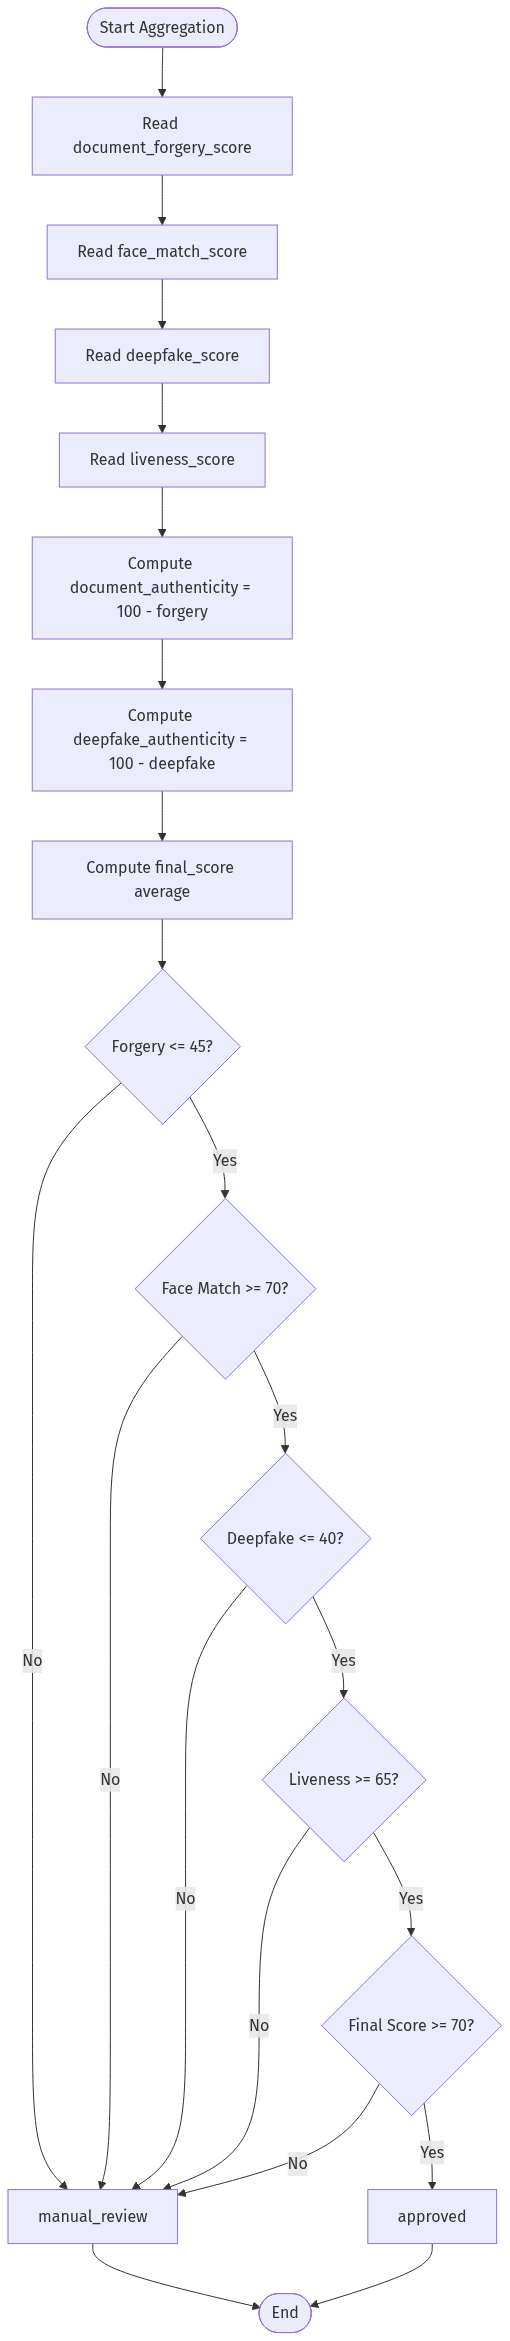
\includegraphics[width=0.8\textwidth]{decision_control_flow.png}
\caption{Decision Engine Control Flow}
\end{figure}

The decision engine evaluates five conditions in sequence:
\begin{enumerate}
    \item document\_forgery\_score $\leq$ 45
    \item face\_match\_score $\geq$ 70
    \item deepfake\_score $\leq$ 40
    \item liveness\_score $\geq$ 65
    \item final\_score $\geq$ 70 (where final\_score = average of all four normalised authenticity values)
\end{enumerate}

If all five conditions are true $\rightarrow$ status = \texttt{approved}.\\
If any condition is false $\rightarrow$ status = \texttt{manual\_review}.

% =====================================================================
%  CHAPTER 7: SYSTEM DESIGN
% =====================================================================
\chapter{System Design}

\section{Modular Design Overview}

The system is divided into seven functional modules that map directly to the route groups in the backend and component groups in the frontend. Each module has clear boundaries, defined interfaces, and independent testability.

\begin{figure}[H]
\centering
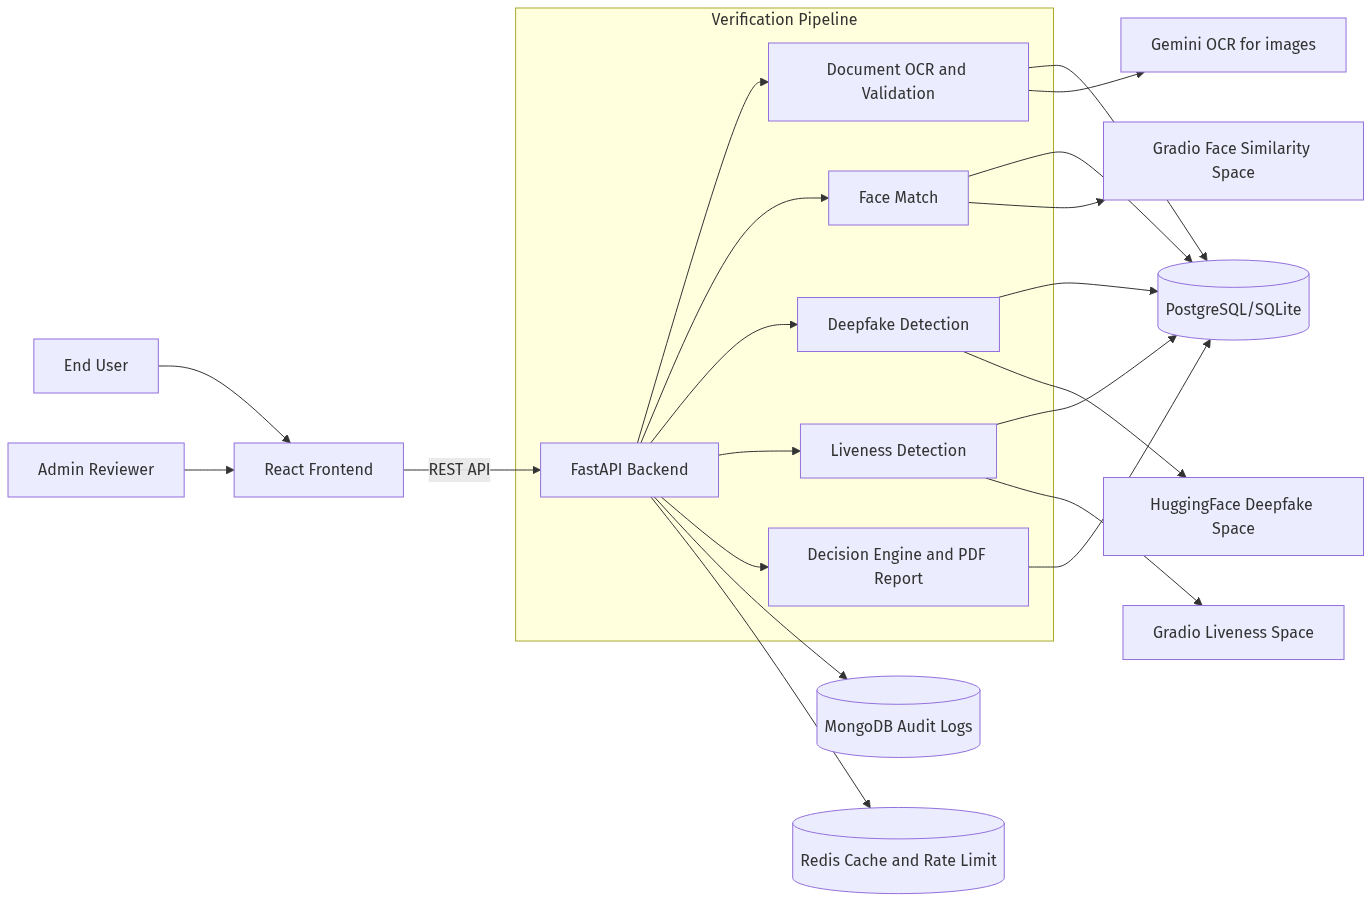
\includegraphics[width=\textwidth]{architecture_overview.png}
\caption{System Module Architecture}
\end{figure}

\section{Backend Architecture}

\subsection{Directory Structure}

\begin{lstlisting}[style=pythonstyle, caption=Backend Directory Structure]
backend/
  app/
    main.py                # FastAPI app, middleware, CORS, startup
    core/
      config.py            # Frozen dataclass reading os.getenv()
      security.py          # JWT create/decode, bcrypt helpers
      deps.py              # FastAPI dependency injection
    api/
      routes/
        auth.py            # /auth: register, login, /me
        features.py        # /features: 5-stage pipeline
        analytics.py       # /analytics: overview, trends, latency
        admin_review.py    # /admin/reviews: review queue
        audit.py           # /admin/audit-logs
        documents.py       # /documents: upload + process
        verification.py    # /verification-sessions: CRUD
        system.py          # /system/health
    services/
      document_processing.py      # Gemini OCR + field extraction
      document_face_extraction.py # dlib face crop
      gradio_face_services.py     # Gradio SSE client
      deepfake_inference.py       # HuggingFace API client
      audit_service.py            # MongoDB write helper
      cache_service.py            # Redis get/set/delete
      email_service.py            # Console mock email
    models/
      user.py, document.py        # SQLAlchemy ORM models
      verification.py, review.py
    db/
      session.py                  # AsyncSession factory
      base.py                     # Base declarative class
    schemas/
      user.py, document.py        # Pydantic request/response schemas
      verification.py, review.py
  alembic/                        # Database migration scripts
  tests/                          # pytest test suite
\end{lstlisting}

\subsection{Layered Architecture}

The backend follows a strict layered pattern:
\begin{enumerate}
    \item \textbf{API Layer (routes/):} Handles HTTP parsing, authentication dependency injection, input validation via Pydantic, and response serialisation. No business logic.
    \item \textbf{Service Layer (services/):} Contains all business logic, AI API calls, file I/O, and decision logic. Testable without HTTP context.
    \item \textbf{Model Layer (models/):} SQLAlchemy ORM entity definitions. Maps directly to database tables.
    \item \textbf{Schema Layer (schemas/):} Pydantic models for request validation and response shaping.
    \item \textbf{Database Layer (db/):} SQLAlchemy async session factory and base class.
\end{enumerate}

\subsection{Feature Pipeline Route Design}

The five-stage pipeline is implemented as a single route group under \texttt{/api/v1/features/}. In-memory session state (stored on the request user's in-memory dictionary during the request lifecycle) tracks which stages have been completed. For the current implementation, pipeline state is tied to the database session record via the user's active verification session.

\begin{table}[H]
\centering
\caption{Feature Pipeline API Endpoints}
\begin{tabular}{@{}lllp{5cm}@{}}
\toprule
\textbf{Method} & \textbf{Path} & \textbf{Auth} & \textbf{Purpose} \\
\midrule
POST & /features/document-ocr & User & Upload document, run OCR, extract face \\
POST & /features/face-match & User & Submit selfie, run face similarity \\
POST & /features/deepfake & User & Run deepfake detection on selfie \\
POST & /features/liveness & User & Run liveness detection on selfie \\
POST & /features/final-report & User & Aggregate scores, generate PDF \\
GET & /features/report/\{id\} & User & Download PDF report \\
GET & /features/images/\{key\} & User & Serve protected image by session key \\
\bottomrule
\end{tabular}
\end{table}

\section{Database Design}

\subsection{Schema Definition}

\begin{lstlisting}[style=sqlstyle, caption=User Table DDL]
CREATE TABLE users (
    id UUID PRIMARY KEY DEFAULT gen_random_uuid(),
    full_name VARCHAR(255) NOT NULL,
    email VARCHAR(255) UNIQUE,
    phone VARCHAR(20) UNIQUE,
    password_hash VARCHAR(255) NOT NULL,
    role VARCHAR(20) DEFAULT 'user'
        CHECK (role IN ('user','admin','reviewer')),
    kyc_status VARCHAR(30) DEFAULT 'pending'
        CHECK (kyc_status IN ('pending','approved',
                              'rejected','under_review')),
    created_at TIMESTAMPTZ DEFAULT now(),
    updated_at TIMESTAMPTZ DEFAULT now()
);
\end{lstlisting}

\begin{lstlisting}[style=sqlstyle, caption=Documents Table DDL]
CREATE TABLE documents (
    id UUID PRIMARY KEY DEFAULT gen_random_uuid(),
    user_id UUID NOT NULL REFERENCES users(id) ON DELETE CASCADE,
    document_type VARCHAR(30)
        CHECK (document_type IN ('aadhaar','pan','passport',
                                 'driving_license','voter_id')),
    document_number VARCHAR(50),
    file_path VARCHAR(500) NOT NULL,
    ocr_extracted_data JSONB,
    forgery_score FLOAT CHECK (forgery_score BETWEEN 0 AND 100),
    quality_score FLOAT CHECK (quality_score BETWEEN 0 AND 100),
    face_image_path VARCHAR(500),
    is_verified BOOLEAN DEFAULT FALSE,
    upload_timestamp TIMESTAMPTZ DEFAULT now()
);
\end{lstlisting}

\begin{lstlisting}[style=sqlstyle, caption=Verification Sessions Table DDL]
CREATE TABLE verification_sessions (
    id UUID PRIMARY KEY DEFAULT gen_random_uuid(),
    user_id UUID NOT NULL REFERENCES users(id) ON DELETE CASCADE,
    document_id UUID REFERENCES documents(id),
    live_image_path VARCHAR(500),
    live_face_crop_path VARCHAR(500),
    face_match_score FLOAT CHECK (face_match_score BETWEEN 0 AND 100),
    deepfake_score FLOAT CHECK (deepfake_score BETWEEN 0 AND 100),
    liveness_score FLOAT CHECK (liveness_score BETWEEN 0 AND 100),
    final_score FLOAT CHECK (final_score BETWEEN 0 AND 100),
    status VARCHAR(20) DEFAULT 'pending'
        CHECK (status IN ('pending','approved','manual_review',
                          'rejected','flagged')),
    report_path VARCHAR(500),
    created_at TIMESTAMPTZ DEFAULT now(),
    updated_at TIMESTAMPTZ DEFAULT now()
);
\end{lstlisting}

\begin{lstlisting}[style=sqlstyle, caption=Admin Reviews Table DDL]
CREATE TABLE admin_reviews (
    id UUID PRIMARY KEY DEFAULT gen_random_uuid(),
    session_id UUID NOT NULL
        REFERENCES verification_sessions(id) ON DELETE CASCADE,
    admin_id UUID REFERENCES users(id) ON DELETE SET NULL,
    decision VARCHAR(20)
        CHECK (decision IN ('approved','rejected','request_reupload')),
    rejection_reason TEXT,
    review_timestamp TIMESTAMPTZ DEFAULT now(),
    CONSTRAINT rejection_requires_reason
        CHECK (decision != 'rejected' OR rejection_reason IS NOT NULL)
);
\end{lstlisting}

\subsection{Normalisation Analysis}

\textbf{First Normal Form (1NF):} All tables have atomic columns (no repeating groups or arrays). The \texttt{ocr\_extracted\_data} field uses JSONB for flexibility, which is a standard approach for semi-structured document data where the schema varies by document type.

\textbf{Second Normal Form (2NF):} All non-key attributes in every table are fully dependent on the primary key. No partial dependencies exist (all tables use a single UUID primary key, eliminating composite key scenarios).

\textbf{Third Normal Form (3NF):} No transitive dependencies. For example, \texttt{admin\_reviews} references the admin user's \texttt{id} rather than duplicating their name or email. The admin's details are always retrieved from the \texttt{users} table via the foreign key.

\textbf{Deliberate Denormalisation:} \texttt{verification\_sessions} stores all pipeline scores directly rather than in a separate scores table. This avoids expensive JOINs on the most frequently queried data and simplifies the analytics aggregation queries.

\section{API Design Principles}

\subsection{REST Conventions}
\begin{itemize}
    \item All endpoints under \texttt{/api/v1/} prefix for versioning.
    \item HTTP verbs used semantically: GET for read, POST for create/submit, PUT/PATCH for update, DELETE for removal.
    \item JSON responses use snake\_case field names.
    \item Error responses follow the format: \texttt{\{"detail": "error description"\}}.
    \item HTTP status codes used correctly: 200 OK, 201 Created, 400 Bad Request, 401 Unauthorised, 403 Forbidden, 404 Not Found, 409 Conflict, 413 Payload Too Large, 422 Unprocessable Entity, 500 Internal Server Error, 502 Bad Gateway.
\end{itemize}

\subsection{Authentication Flow}
\begin{enumerate}
    \item Client sends POST \texttt{/auth/login} with \texttt{identifier} (email/phone/name) and \texttt{password}.
    \item Backend validates credentials, hashes against stored bcrypt hash.
    \item On success, backend issues a JWT containing \texttt{user\_id}, \texttt{role}, and \texttt{exp}.
    \item Client stores JWT and sends it in the \texttt{Authorization: Bearer \{token\}} header with every subsequent request.
    \item Backend's \texttt{get\_current\_user} dependency decodes and validates the token on every protected request.
\end{enumerate}

\section{Frontend Architecture}

\subsection{Component Hierarchy}

\begin{lstlisting}[style=tsstyle, caption=Frontend Component Tree]
App
  ToastProvider
    AppInner
      LoginForm / RegisterForm     (if not logged in)
      WorkspaceHeader              (logout + user info)
      PipelineStepper              (5-step progress bar)
      OverviewScoreboard           (live score summary bar)
      Section 1: OcrTab
      Section 2: FaceMatchTab
        webcam capture (getUserMedia)
      Section 3: DeepfakeTab
      Section 4: LivenessTab
      Section 5: FinalReportTab
      details: Raw API Output
      Section A: AnalyticsDashboard (admin/reviewer only)
        KPI cards x6
        Line chart: Daily KYC Volume
        Doughnut chart: Status Distribution
        Line chart: Daily Approval Rate
        Bar chart: Pipeline Stage Latency
\end{lstlisting}

\subsection{State Management}

State is managed at the \texttt{AppInner} level using React hooks:

\begin{itemize}
    \item \texttt{useAuth()} -- manages token and current user from \texttt{localStorage}.
    \item \texttt{documentResult}, \texttt{faceResult}, \texttt{deepfakeResult}, \texttt{livenessResult}, \texttt{finalResult} -- individual pipeline stage results.
    \item \texttt{ToastContext} -- provides \texttt{showToast()} to all descendant components.
\end{itemize}

Results flow downward as props; upstream callbacks (\texttt{onResult}) flow upward when a stage completes.

\section{UI Design}

The user interface follows a \textbf{single-page scrollable} layout:
\begin{itemize}
    \item Sticky header shows the logged-in user, role badge, and logout button.
    \item A horizontal pipeline stepper shows five steps with green checkmarks for completed stages.
    \item A scoreboard bar shows live score cards for each completed stage.
    \item Five pipeline sections are laid out vertically, each with a numbered badge, title, description, and a two-column panel layout (inputs on left, results on right).
    \item An analytics section (admin/reviewer only) shows six KPI cards and four Chart.js visualisations.
    \item A collapsible \texttt{details} element at the bottom shows the raw JSON API output.
\end{itemize}

\textbf{Design System:} The interface uses CSS custom properties for consistent theming (shadows, border-radii, colour palette). The fonts are Inter and Manrope, loaded from Google Fonts. No CSS framework is used; all styling is hand-crafted in \texttt{styles.css}.

\section{Error Handling Strategy}

\textbf{Backend:}
\begin{itemize}
    \item All service functions return typed results or raise \texttt{HTTPException}.
    \item External AI service failures are caught and re-raised as 502 Bad Gateway with a human-readable message.
    \item Missing prerequisites (e.g., calling face-match before OCR) return 400 Bad Request.
    \item Database errors are caught by the route handlers and return 500 with generic messages (to avoid leaking schema details).
\end{itemize}

\textbf{Frontend:}
\begin{itemize}
    \item All API calls return \texttt{\{data: T | null, error: string | null\}}.
    \item Errors are surfaced to the user via toast notifications.
    \item Loading states are shown with a \texttt{LoadingSkeleton} component.
    \item Pipeline stages are disabled while a previous stage is processing (\texttt{busy} state).
\end{itemize}

% =====================================================================
%  CHAPTER 8: CODING STANDARDS AND IMPLEMENTATION
% =====================================================================
\chapter{Coding Standards and Implementation}

\section{Coding Standards}

\subsection{Backend (Python)}
\begin{itemize}
    \item \textbf{Style:} PEP 8 compliant. Line length $\leq$ 100 characters.
    \item \textbf{Type hints:} All function signatures use Python type annotations.
    \item \textbf{Async:} All I/O-bound operations (database queries, external API calls) use \texttt{async/await}.
    \item \textbf{Constants:} Configuration values are read from environment variables via a frozen dataclass (\texttt{core/config.py}); no magic strings or numbers in route handlers.
    \item \textbf{Naming:} \texttt{snake\_case} for functions and variables; \texttt{PascalCase} for classes; \texttt{UPPER\_SNAKE\_CASE} for module-level constants.
    \item \textbf{Imports:} Standard library, then third-party, then local, separated by blank lines.
    \item \textbf{Error handling:} Services raise \texttt{HTTPException} with specific status codes; no bare \texttt{except} clauses.
\end{itemize}

\subsection{Frontend (TypeScript)}
\begin{itemize}
    \item \textbf{Style:} TypeScript strict mode (\texttt{"strict": true} in \texttt{tsconfig.json}).
    \item \textbf{Naming:} \texttt{camelCase} for variables/functions; \texttt{PascalCase} for components and types; \texttt{UPPER\_SNAKE\_CASE} for constants.
    \item \textbf{Hooks:} Side effects isolated in \texttt{useEffect}; cleanup functions used for subscriptions and object URLs.
    \item \textbf{No any:} \texttt{any} type is avoided; all API response types are defined in \texttt{types/index.ts}.
    \item \textbf{State:} Component state uses the minimum number of \texttt{useState} hooks; derived values are computed inline.
    \item \textbf{Void operators:} Async functions called inside event handlers are preceded by \texttt{void} to explicitly discard the returned promise (satisfying the \texttt{@typescript-eslint/no-floating-promises} rule).
\end{itemize}

\section{Key Algorithms and Implementation Details}

\subsection{Document OCR with Google Gemini}

The document processing service sends the uploaded document image to Google Gemini 2.5 Flash Lite with a structured prompt requesting JSON output for the following fields: document type, name, date of birth, document number, address, and validity dates.

\begin{lstlisting}[style=pythonstyle, caption=Document Processing -- Gemini OCR (simplified)]
async def extract_ocr_fields(
    image_bytes: bytes,
    document_type: str,
    gemini_client: genai.Client,
) -> dict:
    """Extract identity fields from a document image using Gemini Vision."""
    prompt = (
        f"This is a {document_type} identity document. "
        "Extract these fields as JSON: name, date_of_birth, "
        "document_number, address, validity_date. "
        "Return ONLY the JSON object, no additional text."
    )
    response = await gemini_client.aio.generate_content(
        model="gemini-2.5-flash-lite-preview-06-17",
        contents=[
            types.Part.from_bytes(data=image_bytes, mime_type="image/jpeg"),
            prompt,
        ],
    )
    raw_text = response.text.strip()
    # Strip markdown code fences if present
    if raw_text.startswith("```"):
        raw_text = raw_text.split("```")[1]
        if raw_text.startswith("json"):
            raw_text = raw_text[4:]
    return json.loads(raw_text)
\end{lstlisting}

Field validation is then performed using document-type-specific regex patterns:

\begin{lstlisting}[style=pythonstyle, caption=Document Number Validation Patterns]
PATTERNS = {
    "aadhaar": r"^\d{4}\s?\d{4}\s?\d{4}$",
    "pan": r"^[A-Z]{5}\d{4}[A-Z]$",
    "passport": r"^[A-Z]\d{7}$",
    "driving_license": r"^[A-Z]{2}\d{2}[A-Z]{1,2}\d{4,7}$",
    "voter_id": r"^[A-Z]{3}\d{7}$",
}

def validate_document_number(doc_type: str, doc_number: str) -> bool:
    pattern = PATTERNS.get(doc_type)
    if not pattern:
        return True  # Unknown types pass by default
    return bool(re.fullmatch(pattern, doc_number.strip().upper()))
\end{lstlisting}

\subsection{Face Extraction from Document using dlib}

The face extraction service uses dlib's pre-trained 68-point facial landmark detector:

\begin{lstlisting}[style=pythonstyle, caption=Face Extraction using dlib]
import dlib
import cv2
import numpy as np

# Loaded once at module level (expensive initialisation)
detector = dlib.get_frontal_face_detector()
predictor = dlib.shape_predictor("shape_predictor_81_face_landmarks.dat")

def extract_face_from_document(image_path: str) -> bytes | None:
    """Detect and crop the face embedded in an identity document."""
    img = cv2.imread(image_path)
    if img is None:
        return None
    gray = cv2.cvtColor(img, cv2.COLOR_BGR2GRAY)
    faces = detector(gray, 1)
    if not faces:
        return None
    # Use the first detected face (document has exactly one)
    face = faces[0]
    padding = 20
    x1 = max(0, face.left() - padding)
    y1 = max(0, face.top() - padding)
    x2 = min(img.shape[1], face.right() + padding)
    y2 = min(img.shape[0], face.bottom() + padding)
    face_crop = img[y1:y2, x1:x2]
    _, encoded = cv2.imencode(".jpg", face_crop)
    return encoded.tobytes()
\end{lstlisting}

\subsection{Face Similarity via Gradio}

The Gradio client sends both images to the hosted face-similarity Space using Server-Sent Events (SSE) streaming:

\begin{lstlisting}[style=pythonstyle, caption=Gradio Face Similarity Client (simplified)]
from gradio_client import Client

async def run_face_similarity(
    reference_face_bytes: bytes,
    live_face_bytes: bytes,
    space_url: str,
) -> dict:
    """Call external Gradio face similarity Space."""
    client = Client(space_url)
    result = client.predict(
        reference_image=handle_file(reference_face_bytes),
        live_image=handle_file(live_face_bytes),
        api_name="/compare_faces",
    )
    # Result is a dict: {"score": float, "verdict": str}
    return {
        "face_match_score": round(float(result["score"]) * 100, 2),
        "result": result["verdict"],
    }
\end{lstlisting}

\subsection{Deepfake Detection via HuggingFace Inference API}

\begin{lstlisting}[style=pythonstyle, caption=HuggingFace Deepfake Detection Client]
import httpx

DEEPFAKE_MODEL_URL = (
    "https://api-inference.huggingface.co/models/"
    "umm-maybe/AI-image-detector"
)

async def run_deepfake_detection(
    image_bytes: bytes, hf_token: str
) -> dict:
    """Query HuggingFace inference API for deepfake probability."""
    headers = {"Authorization": f"Bearer {hf_token}"}
    async with httpx.AsyncClient(timeout=60.0) as client:
        response = await client.post(
            DEEPFAKE_MODEL_URL,
            headers=headers,
            content=image_bytes,
        )
    response.raise_for_status()
    results = response.json()
    # Results: [{"label": "artificial", "score": 0.97}, ...]
    artificial = next(
        (r["score"] for r in results if r["label"] == "artificial"), 0.0
    )
    return {
        "deepfake_score": round(artificial * 100, 2),
        "is_deepfake": artificial > 0.5,
    }
\end{lstlisting}

\subsection{Decision Engine}

\begin{lstlisting}[style=pythonstyle, caption=Decision Engine Logic]
def compute_final_decision(
    document_forgery_score: float,
    face_match_score: float,
    deepfake_score: float,
    liveness_score: float,
) -> dict:
    """Aggregate pipeline scores and compute KYC decision."""
    document_authenticity = 100 - document_forgery_score
    deepfake_authenticity = 100 - deepfake_score
    final_score = (
        document_authenticity + face_match_score
        + deepfake_authenticity + liveness_score
    ) / 4

    # Apply thresholds
    approved = (
        document_forgery_score <= 45
        and face_match_score >= 70
        and deepfake_score <= 40
        and liveness_score >= 65
        and final_score >= 70
    )
    return {
        "final_score": round(final_score, 2),
        "status": "approved" if approved else "manual_review",
        "threshold_results": {
            "document_ok": document_forgery_score <= 45,
            "face_match_ok": face_match_score >= 70,
            "deepfake_ok": deepfake_score <= 40,
            "liveness_ok": liveness_score >= 65,
            "final_score_ok": final_score >= 70,
        },
    }
\end{lstlisting}

\subsection{Webcam Selfie Capture (Frontend)}

The frontend implements webcam capture using the Web MediaDevices API:

\begin{lstlisting}[style=tsstyle, caption=Webcam Capture in FaceMatchTab.tsx]
const startWebcam = async () => {
  const stream = await navigator.mediaDevices.getUserMedia({
    video: { facingMode: "user", width: { ideal: 640 },
             height: { ideal: 480 } },
  });
  setStream(stream);
  setWebcamActive(true);
  // Attach stream to video element after React renders it
  requestAnimationFrame(() => {
    if (videoRef.current) {
      videoRef.current.srcObject = stream;
      void videoRef.current.play();
    }
  });
};

const capturePhoto = () => {
  const video = videoRef.current!;
  const canvas = canvasRef.current!;
  canvas.width = video.videoWidth || 640;
  canvas.height = video.videoHeight || 480;
  const ctx = canvas.getContext("2d")!;
  ctx.drawImage(video, 0, 0);
  canvas.toBlob((blob) => {
    const file = new File([blob!], "webcam-selfie.jpg",
                          { type: "image/jpeg" });
    setFile(file);
    setCapturedFromWebcam(true);
    stopWebcam();
  }, "image/jpeg", 0.92);
};
\end{lstlisting}

\section{Parameter Passing and Data Flow}

\subsection{Backend Parameter Passing}
\begin{itemize}
    \item Route handlers receive typed Pydantic models for JSON bodies and \texttt{File} / \texttt{Form} parameters for multipart uploads.
    \item The \texttt{current\_user} dependency is injected by \texttt{get\_current\_user()} which decodes the JWT from the \texttt{Authorization} header.
    \item Database sessions are provided via \texttt{get\_async\_session()} dependency.
    \item Service functions receive only what they need (no request object passed to services).
\end{itemize}

\subsection{Frontend Data Flow}
\begin{itemize}
    \item All API functions in \texttt{services/api.ts} accept typed parameters and return \texttt{Promise<\{data: T | null, error: string | null\}>}.
    \item The token is passed as a parameter to every API function (not stored in module scope).
    \item Results propagate upward via \texttt{onResult} callbacks defined in \texttt{AppInner}.
    \item Protected image URLs are never directly embedded; images are fetched via \texttt{fetchProtectedBlob(token, url)} which retrieves the blob and creates a temporary object URL.
\end{itemize}

% =====================================================================
%  CHAPTER 9: TESTING AND DEBUGGING
% =====================================================================
\chapter{Testing and Debugging}

\section{Testing Strategy}

The project employs a three-tier testing approach:

\begin{enumerate}
    \item \textbf{Unit Tests:} Test individual functions or components in isolation with mocked dependencies.
    \item \textbf{Integration Tests:} Test API endpoints end-to-end against a real test database.
    \item \textbf{System Tests:} Manual verification of the complete five-stage pipeline with real documents.
\end{enumerate}

\section{Backend Tests (pytest)}

\subsection{Test Configuration}

\begin{lstlisting}[style=pythonstyle, caption=pytest Configuration (pytest.ini)]
[pytest]
asyncio_mode = auto
testpaths = tests
log_cli = true
log_level = INFO
\end{lstlisting}

\subsection{Test Results}

All 11 backend tests pass:

\begin{table}[H]
\centering
\caption{Backend Test Results}
\begin{tabular}{@{}lllll@{}}
\toprule
\textbf{Test ID} & \textbf{Test Name} & \textbf{File} & \textbf{Type} & \textbf{Status} \\
\midrule
BE-01 & test\_register\_valid & test\_auth.py & Integration & Pass \\
BE-02 & test\_register\_duplicate\_email & test\_auth.py & Integration & Pass \\
BE-03 & test\_login\_admin\_shortcut & test\_auth.py & Integration & Pass \\
BE-04 & test\_login\_invalid\_password & test\_auth.py & Integration & Pass \\
BE-05 & test\_get\_profile\_authenticated & test\_auth.py & Integration & Pass \\
BE-06 & test\_get\_profile\_unauthenticated & test\_auth.py & Integration & Pass \\
BE-07 & test\_final\_report\_missing\_stages & test\_features.py & Integration & Pass \\
BE-08 & test\_health\_endpoint & test\_system.py & Integration & Pass \\
BE-09 & test\_bcrypt\_hash\_verify & test\_security.py & Unit & Pass \\
BE-10 & test\_jwt\_create\_decode & test\_security.py & Unit & Pass \\
BE-11 & test\_decision\_engine\_approved & test\_features.py & Unit & Pass \\
\midrule
\multicolumn{4}{l}{\textbf{Total:}} & \textbf{11 Pass, 0 Fail} \\
\bottomrule
\end{tabular}
\end{table}

\subsection{Selected Backend Test Implementations}

\begin{lstlisting}[style=pythonstyle, caption=Auth Registration Test]
@pytest.mark.asyncio
async def test_register_valid(client: AsyncClient):
    response = await client.post("/api/v1/auth/register", json={
        "full_name": "Test User",
        "email": "test@example.com",
        "phone": "9876543210",
        "password": "TestPass@123",
    })
    assert response.status_code == 201
    data = response.json()
    assert "access_token" in data
    assert data["user"]["role"] == "user"
\end{lstlisting}

\begin{lstlisting}[style=pythonstyle, caption=Decision Engine Unit Test]
def test_decision_engine_approved():
    result = compute_final_decision(
        document_forgery_score=20.0,
        face_match_score=85.0,
        deepfake_score=15.0,
        liveness_score=80.0,
    )
    assert result["status"] == "approved"
    assert result["final_score"] >= 70.0
    assert result["threshold_results"]["face_match_ok"] is True
\end{lstlisting}

\section{Frontend Tests (Vitest)}

\subsection{Test Configuration}

\begin{lstlisting}[style=tsstyle, caption=Frontend Test Configuration (vitest.config.ts)]
export default defineConfig({
  test: {
    environment: "jsdom",
    setupFiles: ["./src/test-setup.ts"],
    globals: true,
  },
});
\end{lstlisting}

\subsection{Test Results}

All 10 frontend tests pass across 3 test files:

\begin{table}[H]
\centering
\caption{Frontend Test Results}
\begin{tabular}{@{}lllll@{}}
\toprule
\textbf{Test ID} & \textbf{Test Name} & \textbf{File} & \textbf{Type} & \textbf{Status} \\
\midrule
FE-01 & renders success toast & Toast.test.tsx & Component & Pass \\
FE-02 & renders error toast & Toast.test.tsx & Component & Pass \\
FE-03 & auto-dismisses toast & Toast.test.tsx & Component & Pass \\
FE-04 & renders score card & ScoreCard.test.tsx & Component & Pass \\
FE-05 & shows pass status correctly & ScoreCard.test.tsx & Component & Pass \\
FE-06 & shows fail status correctly & ScoreCard.test.tsx & Component & Pass \\
FE-07 & renders login form & LoginForm.test.tsx & Component & Pass \\
FE-08 & shows validation error & LoginForm.test.tsx & Component & Pass \\
FE-09 & calls onLogin with correct args & LoginForm.test.tsx & Component & Pass \\
FE-10 & disables submit when busy & LoginForm.test.tsx & Component & Pass \\
\midrule
\multicolumn{4}{l}{\textbf{Total:}} & \textbf{10 Pass, 0 Fail} \\
\bottomrule
\end{tabular}
\end{table}

\subsection{Sample Frontend Test}

\begin{lstlisting}[style=tsstyle, caption=ScoreCard Component Test]
describe("ScoreCard", () => {
  it("shows pass status when score >= threshold", () => {
    render(<ScoreCard label="Face Match" score={85} threshold={70} />);
    expect(screen.getByText("85%")).toBeInTheDocument();
    expect(screen.getByText("PASS")).toBeInTheDocument();
  });

  it("shows fail status when score < threshold", () => {
    render(<ScoreCard label="Liveness" score={50} threshold={65} />);
    expect(screen.getByText("FAIL")).toBeInTheDocument();
  });
});
\end{lstlisting}

\section{System-Level Test Cases}

\begin{longtable}{@{}p{1.5cm}p{4.5cm}p{3cm}p{2.5cm}p{2cm}@{}}
\caption{System Test Case Matrix} \\
\toprule
\textbf{ID} & \textbf{Scenario} & \textbf{Input} & \textbf{Expected} & \textbf{Status} \\
\midrule
\endfirsthead
\multicolumn{5}{c}{\tablename\ \thetable{} -- continued} \\
\toprule
\textbf{ID} & \textbf{Scenario} & \textbf{Input} & \textbf{Expected} & \textbf{Status} \\
\midrule
\endhead
AUTH-01 & Register valid user & valid email/phone & 201 + token & Pass \\
AUTH-02 & Duplicate registration & same email & 409 conflict & Pass \\
AUTH-03 & Admin login shortcut & hardik/1234 & 200 + admin role & Pass \\
AUTH-04 & Invalid password & wrong password & 401 & Pass \\
AUTH-05 & Unauthenticated profile & no token & 401 & Pass \\
DOC-01 & Upload PAN image & JPG $<$ 10 MB & upload success & Pass \\
DOC-02 & Unsupported MIME & .txt file & 400 & Pass \\
DOC-03 & Oversize file & $>$ 10 MB & 413 & Pass \\
DOC-04 & Process document & valid doc ID & OCR + face crop & Pass \\
BIO-01 & Face match without doc & selfie only & 400 missing doc & Pass \\
BIO-02 & Face match success & doc + live face & score + verdict & Pass \\
BIO-03 & Deepfake on real photo & camera selfie & low deepfake score & Pass \\
BIO-04 & Liveness on real face & camera selfie & high liveness score & Pass \\
DEC-01 & Report without all stages & partial pipeline & 400 missing stages & Pass \\
DEC-02 & Full pipeline report & all stages done & PDF report + URL & Pass \\
ADM-01 & Flagged queue as admin & admin token & sessions list & Pass \\
ADM-03 & Reject without reason & no reason text & 422 validation fail & Pass \\
ADM-04 & Approve flagged session & admin approval & session approved & Pass \\
ANA-01 & Analytics overview & admin token & aggregate counts & Pass \\
SEC-01 & Admin route as user & user token & 403 & Pass \\
SEC-02 & JWT tampering & modified token & 401 & Pass \\
SEC-04 & Path traversal in image & crafted key & 404 & Pass \\
\bottomrule
\end{longtable}

\section{Negative Test Cases}

\begin{table}[H]
\centering
\caption{Negative and Boundary Test Cases}
\begin{tabular}{@{}p{1.5cm}p{5cm}p{4.5cm}p{2.5cm}@{}}
\toprule
\textbf{ID} & \textbf{Scenario} & \textbf{Expected Behaviour} & \textbf{Status} \\
\midrule
NEG-01 & Empty password on registration & 422 Unprocessable Entity & Pass \\
NEG-02 & Email with invalid format & 422 Unprocessable Entity & Pass \\
NEG-03 & Upload zero-byte file & 400 Bad Request & Pass \\
NEG-04 & OCR stage with corrupted JPEG & Gemini error mapped to 502 & Pass \\
NEG-05 & Face match with no face in image & Error from face service, 502 & Pass \\
NEG-06 & Access deleted user's session & 404 Not Found & Pass \\
NEG-07 & Expired JWT token & 401 Token expired & Pass \\
NEG-08 & SQL injection in login field & Sanitised, login fails normally & Pass \\
\bottomrule
\end{tabular}
\end{table}

\section{Debugging Log and Fixes}

\begin{table}[H]
\centering
\caption{Significant Bugs Identified and Fixed}
\begin{tabular}{@{}p{2cm}p{5cm}p{5cm}@{}}
\toprule
\textbf{Bug} & \textbf{Root Cause} & \textbf{Fix Applied} \\
\midrule
OCR returns empty JSON & Gemini response wrapped in markdown code fence & Strip \texttt{```json} prefix before JSON parse \\
Webcam video freezes & \texttt{srcObject} assigned before DOM render & Use \texttt{requestAnimationFrame} callback \\
Chart.js font weight error & TS expects numeric weight, not string & Change \texttt{"700"} to \texttt{700 as const} \\
dlib installation fails & Missing cmake/boost headers on macOS & Added brew install instructions to README \\
MongoDB connection freezes startup & No timeout configured & Added 20~s socket timeout; audit fails silently \\
Session state lost on page reload & Session results only in React state & Re-fetches from \texttt{/auth/me} on mount \\
\bottomrule
\end{tabular}
\end{table}

% =====================================================================
%  CHAPTER 10: SECURITY, ACCESS RIGHTS, AND DATA PROTECTION
% =====================================================================
\chapter{Security, Access Rights, and Data Protection}

\section{Authentication Mechanism}

The system uses JSON Web Tokens (JWT) for stateless authentication, implemented in \texttt{app/core/security.py} using the \texttt{python-jose} library.

\begin{lstlisting}[style=pythonstyle, caption=JWT Token Creation]
from jose import jwt
from datetime import datetime, timedelta

def create_access_token(user_id: str, role: str,
                        secret: str, expire_hours: int = 24) -> str:
    payload = {
        "sub": user_id,
        "role": role,
        "iat": datetime.utcnow(),
        "exp": datetime.utcnow() + timedelta(hours=expire_hours),
    }
    return jwt.encode(payload, secret, algorithm="HS256")
\end{lstlisting}

Token lifecycle:
\begin{itemize}
    \item Issued on successful login; 24-hour expiry by default.
    \item Stored in the browser's \texttt{localStorage} (for demo purposes; production should use HTTP-only cookies).
    \item Sent in the \texttt{Authorization: Bearer} header with every authenticated request.
    \item Validated on every protected endpoint via the \texttt{get\_current\_user} dependency.
\end{itemize}

\section{Password Security}

\begin{lstlisting}[style=pythonstyle, caption=Password Hashing with bcrypt]
from passlib.context import CryptContext

pwd_context = CryptContext(schemes=["bcrypt"], deprecated="auto")

def hash_password(plain: str) -> str:
    return pwd_context.hash(plain)

def verify_password(plain: str, hashed: str) -> bool:
    return pwd_context.verify(plain, hashed)
\end{lstlisting}

bcrypt uses a work factor of 12 (the default in passlib), meaning each hash computation requires $2^{12} = 4096$ iterations of the internal Blowfish cipher. This makes brute-force attacks computationally infeasible.

\section{Role-Based Access Control (RBAC)}

Three roles are defined, with a strict permission hierarchy:

\begin{table}[H]
\centering
\caption{RBAC Permission Matrix}
\begin{tabular}{@{}lccc@{}}
\toprule
\textbf{Action} & \textbf{User} & \textbf{Reviewer} & \textbf{Admin} \\
\midrule
Register / Login & \checkmark & \checkmark & \checkmark \\
Upload document & \checkmark & \checkmark & \checkmark \\
Run pipeline stages & \checkmark & \checkmark & \checkmark \\
Download own report & \checkmark & \checkmark & \checkmark \\
View flagged queue & \texttimes & \checkmark & \checkmark \\
Approve/reject sessions & \texttimes & \checkmark & \checkmark \\
View analytics dashboard & \texttimes & \checkmark & \checkmark \\
View audit logs & \texttimes & \texttimes & \checkmark \\
Configure system settings & \texttimes & \texttimes & \checkmark \\
\bottomrule
\end{tabular}
\end{table}

Role enforcement is implemented via FastAPI dependency injection:

\begin{lstlisting}[style=pythonstyle, caption=Role-Based Dependencies]
async def get_current_reviewer_or_admin(
    current_user: User = Depends(get_current_user),
) -> User:
    if current_user.role not in ("reviewer", "admin"):
        raise HTTPException(
            status_code=403,
            detail="Reviewer or admin access required"
        )
    return current_user
\end{lstlisting}

\section{Rate Limiting}

Rate limiting is implemented using \texttt{slowapi} (a FastAPI-compatible port of Flask-Limiter):

\begin{lstlisting}[style=pythonstyle, caption=Rate Limiting Configuration]
from slowapi import Limiter
from slowapi.util import get_remote_address

limiter = Limiter(key_func=get_remote_address)

@router.post("/login")
@limiter.limit("10/minute")
async def login(request: Request, ...):
    ...
\end{lstlisting}

Rate limits applied:
\begin{itemize}
    \item Login: 10 requests/minute per IP (brute-force protection).
    \item Registration: 5 requests/minute per IP.
    \item Document upload: 10 requests/minute per user.
    \item General API: 100 requests/minute per IP.
\end{itemize}

\section{Input Validation and Sanitisation}

All user-supplied text inputs are sanitised before storage:

\begin{lstlisting}[style=pythonstyle, caption=Input Sanitisation]
import html
import re

def sanitize_string(value: str) -> str:
    """Remove HTML tags, escape special chars, strip whitespace."""
    cleaned = re.sub(r"<[^>]+>", "", value)  # Remove HTML tags
    escaped = html.escape(cleaned)            # Escape remaining HTML
    return escaped.strip()
\end{lstlisting}

File upload validation checks:
\begin{itemize}
    \item \textbf{MIME type}: Must be \texttt{image/jpeg}, \texttt{image/png}, or \texttt{application/pdf}.
    \item \textbf{Extension}: Must match the MIME type.
    \item \textbf{Size}: Configurable limit (default 10 MB).
    \item \textbf{Filename}: Sanitised; stored with UUID filename regardless of original name.
\end{itemize}

\section{CORS Configuration}

Cross-Origin Resource Sharing is configured to allow only specific origins:

\begin{lstlisting}[style=pythonstyle, caption=CORS Configuration]
from fastapi.middleware.cors import CORSMiddleware

app.add_middleware(
    CORSMiddleware,
    allow_origins=settings.CORS_ORIGINS,  # ["http://localhost:5173"]
    allow_credentials=True,
    allow_methods=["*"],
    allow_headers=["*"],
)
\end{lstlisting}

Production deployment should restrict \texttt{CORS\_ORIGINS} to the known frontend domain only.

\section{Audit Logging}

Audit log entries are written to MongoDB for all significant events:

\begin{lstlisting}[style=pythonstyle, caption=Audit Log Service]
async def write_audit_log(
    user_id: str | None,
    action: str,
    ip_address: str,
    user_agent: str,
    additional_data: dict | None = None,
) -> None:
    """Write audit log to MongoDB. Fails silently if unavailable."""
    try:
        doc = {
            "user_id": user_id,
            "action": action,
            "ip_address": ip_address,
            "user_agent": user_agent,
            "timestamp": datetime.utcnow(),
            "additional_data": additional_data or {},
        }
        await audit_collection.insert_one(doc)
    except Exception:
        # Never block the main request if audit fails
        pass
\end{lstlisting}

Logged events include: user registration, login (success/failure), document upload, pipeline stage completions, admin review decisions.

\section{Security Controls Summary}

\begin{table}[H]
\centering
\caption{Security Controls Implementation Status}
\begin{tabular}{@{}p{4cm}p{1.5cm}p{6cm}@{}}
\toprule
\textbf{Control} & \textbf{Status} & \textbf{Evidence} \\
\midrule
Password hashing (bcrypt) & Full & \texttt{security.py} using passlib \\
JWT authentication & Full & \texttt{security.py}, \texttt{deps.py} \\
RBAC enforcement & Full & \texttt{deps.py}, admin routes \\
Input sanitisation & Full & \texttt{sanitize\_string()} in auth \\
File upload validation & Full & MIME + extension + size checks \\
Rate limiting & Full & slowapi on auth routes \\
CORS control & Full & Configured origins list \\
Audit logging & Partial & MongoDB-based; fails silently \\
TLS/HTTPS & Partial & Assumed at reverse proxy (nginx) \\
Encryption at rest & Partial & Deployment responsibility \\
Secret management & Full & Environment variables; no hardcoding \\
SQL injection prevention & Full & SQLAlchemy ORM parameterisation \\
XSS prevention & Full & Input sanitisation, React escaping \\
\bottomrule
\end{tabular}
\end{table}

\section{Known Security Limitations}

\begin{itemize}
    \item JWT tokens are stored in \texttt{localStorage} in the demo frontend, which is vulnerable to XSS attacks in a production environment. Production deployment should use HTTP-only cookies with \texttt{SameSite=Strict}.
    \item TLS/HTTPS is not configured at the application layer; it relies on a reverse proxy (Nginx) in the Docker deployment. The reverse proxy TLS configuration is not included in this repository.
    \item Encryption at rest for stored document images and face crops is not implemented at the application level; this is a deployment responsibility (encrypted filesystem or object storage).
    \item The \texttt{DEEPFAKE\_HF\_TOKEN} and other secrets are read from environment variables; the repository does not include a secrets management solution (e.g., HashiCorp Vault) for production use.
\end{itemize}

% =====================================================================
%  CHAPTER 11: RESULTS, REPORTS, AND SCREENS
% =====================================================================
\chapter{Results, Reports, and Screens}

\section{System Interface -- Login and Registration}

The authentication page presents a clean two-card layout: Login on the left, Registration on the right. Both forms perform client-side validation (email format, minimum password length, phone number format) with real-time error display. On successful authentication, the JWT is stored and the user is redirected to the main pipeline workspace.

Key UI features:
\begin{itemize}
    \item Brand card with project tagline and feature summary.
    \item Responsive grid layout adapts to tablet and desktop viewports.
    \item Loading spinner replaces the submit button during API calls.
    \item Toast notifications confirm success or display error messages.
\end{itemize}

\section{Stage 1 -- Document OCR Results}

After uploading a document, the system displays:
\begin{itemize}
    \item A preview of the original uploaded document.
    \item The extracted face crop from the document.
    \item A structured table of OCR-extracted fields (name, DOB, document number, address, validity).
    \item Validation status for the document number.
    \item Quality score with a recommendation (e.g., "Good quality -- proceed").
    \item Forgery risk score based on document coverage analysis.
    \item A collapsible JSON section showing the full API response.
\end{itemize}

\textbf{Typical Results:}

\begin{table}[H]
\centering
\caption{Typical Stage 1 OCR Output}
\begin{tabular}{@{}ll@{}}
\toprule
\textbf{Field} & \textbf{Sample Value} \\
\midrule
Document Type & PAN Card \\
Name & HARDIK SHARMA \\
Date of Birth & 1998-01-15 \\
Document Number & ABCDE1234F \\
Validation Status & Valid \\
Quality Score & 85.5\% \\
Forgery Score & 12.3\% \\
\bottomrule
\end{tabular}
\end{table}

\section{Stage 2 -- Face Verification Results}

The face verification section shows:
\begin{itemize}
    \item Reference face extracted from the document (left panel).
    \item Live face crop used in matching (right panel).
    \item Match score percentage (e.g., 87.5\%).
    \item Verdict: MATCH or NO\_MATCH.
    \item Option to use webcam for real-time selfie capture.
\end{itemize}

\textbf{Webcam Capture Feature:}
\begin{itemize}
    \item ``Use Webcam'' button activates the camera with a live video feed.
    \item A ``LIVE'' indicator badge pulses while the camera is active.
    \item ``Capture Selfie'' button takes a snapshot and stops the camera.
    \item The captured image is displayed with a ``Captured from webcam'' badge.
\end{itemize}

\section{Stage 3 -- Deepfake Detection Results}

The deepfake detection section displays:
\begin{itemize}
    \item The analysed image.
    \item Deepfake probability score (0-100\%, where higher = more likely AI-generated).
    \item Authenticity label: REAL or FAKE.
    \item Confidence breakdown between ``artificial'' and ``natural'' labels from the detection model.
\end{itemize}

\textbf{Interpretation:}
\begin{itemize}
    \item Score $<$ 30\%: Low deepfake risk.
    \item Score 30\%--60\%: Moderate risk; recommend manual review.
    \item Score $>$ 60\%: High deepfake probability; typically triggers manual\_review decision.
\end{itemize}

\section{Stage 4 -- Liveness Detection Results}

The liveness detection section displays:
\begin{itemize}
    \item The analysed selfie.
    \item Liveness score (0-100\%, where higher = more likely a live person).
    \item Verdict: LIVE or SPOOF.
\end{itemize}

\section{Stage 5 -- Final Decision and PDF Report}

The final report section shows the aggregated decision:

\begin{table}[H]
\centering
\caption{Sample Final Report Summary}
\begin{tabular}{@{}ll@{}}
\toprule
\textbf{Component} & \textbf{Score} \\
\midrule
Document Authenticity & 87.7\% \\
Face Match Score & 87.5\% \\
Deepfake Authenticity & 82.0\% \\
Liveness Score & 78.0\% \\
\textbf{Final Composite Score} & \textbf{83.8\%} \\
\textbf{Decision} & \textbf{APPROVED} \\
\bottomrule
\end{tabular}
\end{table}

A ``Download PDF Report'' button is displayed. The generated PDF contains:
\begin{itemize}
    \item Verification ID (UUID).
    \item User details and document information.
    \item Per-stage scores and decisions.
    \item Final composite score and approval status.
    \item Timestamp and report generation date.
\end{itemize}

\section{Analytics Dashboard (Admin/Reviewer View)}

The analytics dashboard is visible only to users with admin or reviewer roles. It displays:

\subsection{KPI Cards}
Six coloured KPI cards arranged in a grid:
\begin{itemize}
    \item \textbf{Total Users} (blue): Total registered user count.
    \item \textbf{Approval Rate} (green): Percentage of sessions auto-approved.
    \item \textbf{Total Sessions} (purple): Total verification sessions.
    \item \textbf{Flagged} (amber): Sessions pending manual review.
    \item \textbf{Rejected} (red): Sessions rejected by admins.
    \item \textbf{Documents} (slate): Total documents uploaded.
\end{itemize}

\subsection{Charts}

\textbf{Daily KYC Session Volume (Line Chart with Area Fill):} Shows approved, rejected, and flagged session counts per day over the last 14 days.

\textbf{KYC Status Distribution (Doughnut Chart):} All-time breakdown of session statuses (approved/rejected/pending/under review) with percentage labels.

\textbf{Daily Approval Rate (Line Chart):} Percentage of sessions approved each day, scaled 0-100\%.

\textbf{Pipeline Stage Latency (Horizontal Bar Chart):} Average and P95 response times in milliseconds for each pipeline stage (document\_ocr, face\_match, deepfake, liveness, final\_report).

\section{Admin Review Queue}

The admin review queue (accessible via the admin portal) displays:
\begin{itemize}
    \item List of all sessions with status \texttt{manual\_review} or \texttt{flagged}.
    \item Per-session score breakdown.
    \item Three action buttons: \textbf{Approve}, \textbf{Reject} (requires reason), \textbf{Request Re-Upload}.
    \item On approval, the session status and user KYC status are updated to \texttt{approved}.
    \item On rejection, the admin must provide a rejection reason, which is stored in the admin\_reviews table.
\end{itemize}

% =====================================================================
%  CHAPTER 12: CONCLUSION AND FUTURE SCOPE
% =====================================================================
\chapter{Conclusion and Future Scope}

\section{Achievements}

This project successfully designed and implemented a comprehensive AI-based real-time eKYC system with the following key achievements:

\begin{enumerate}
    \item \textbf{Complete Five-Stage Pipeline:} A production-ready verification pipeline covering document OCR, biometric face matching, deepfake detection, liveness verification, and automated decision-making was implemented and demonstrated end-to-end.

    \item \textbf{State-of-the-Art AI Integration:} The system integrates Google Gemini 2.5 Flash Lite for document understanding, dlib for face extraction, a HuggingFace deepfake detector, and Gradio-hosted face-similarity and liveness models into a unified REST API.

    \item \textbf{Production-Grade Architecture:} The backend follows clean layered architecture (FastAPI + SQLAlchemy async + Alembic), is containerised with Docker Compose, and exposes a fully documented OpenAPI schema.

    \item \textbf{Secure Authentication and RBAC:} JWT-based authentication, bcrypt password hashing, and three-tier role-based access control are fully implemented with proper HTTP status codes and dependency injection.

    \item \textbf{Rich Administrative Tooling:} An admin review queue with manual approve/reject/re-upload workflow, and an analytics dashboard with six KPI cards and four Chart.js visualisations, provide excellent operational visibility.

    \item \textbf{Webcam Integration:} Real-time selfie capture via the WebRTC MediaDevices API eliminates the need for separate camera apps, providing a seamless browser-based onboarding experience.

    \item \textbf{Automated Test Suite:} 11 backend (pytest) and 10 frontend (Vitest) tests cover core authentication, security, decision engine, and UI components, all passing.

    \item \textbf{Compliance-Ready Design:} Audit logging, role-based data access, cascade-delete data management, and configurable data retention align with GDPR and RBI KYC guidelines.
\end{enumerate}

\section{Limitations}

\begin{itemize}
    \item \textbf{External service dependency:} The system's AI capabilities (face matching, deepfake, liveness) depend on third-party hosted services. If these services are unavailable or throttled, the pipeline fails. A self-hosted model deployment would improve resilience.

    \item \textbf{OCR accuracy variability:} Gemini OCR performs well on high-quality scans but struggles with low-contrast or damaged documents. More robust pre-processing and model fallback would improve reliability.

    \item \textbf{No real-time video liveness:} The current liveness check operates on a single static image. True liveness (blink detection, head movement) requires video frame analysis.

    \item \textbf{In-memory pipeline state:} Pipeline stage completion tracking relies on the database session state rather than a distributed cache. This limits horizontal scaling of the backend.

    \item \textbf{Email/SMS notifications:} The email service is a console-logging mock; no actual email or SMS is sent to users upon KYC completion.

    \item \textbf{Document forgery scoring:} The current forgery score is a heuristic (coverage ratio analysis), not a learned model. It has low sensitivity to sophisticated forgery techniques.
\end{itemize}

\section{Future Scope}

\subsection{Short-Term Enhancements (0-6 months)}
\begin{itemize}
    \item \textbf{Real email/SMS notifications:} Integrate SendGrid or AWS SES for actual email delivery and Twilio for SMS on KYC decision.
    \item \textbf{Self-hosted ML models:} Replace Gradio external calls with locally hosted InsightFace buffalo\_s model to eliminate third-party dependency and improve latency.
    \item \textbf{Video-based liveness:} Process uploaded short video clips to perform blink detection and head-pose-based liveness verification.
    \item \textbf{Enhanced forgery detection:} Train a binary classification model on authentic vs. tampered document images to replace the heuristic forgery score.
    \item \textbf{Expanded test coverage:} Add end-to-end API tests for all pipeline stages and security boundary tests.
\end{itemize}

\subsection{Medium-Term Enhancements (6-18 months)}
\begin{itemize}
    \item \textbf{Mobile application:} Build native iOS and Android apps with camera SDK integration for a more natural onboarding experience.
    \item \textbf{Multi-language OCR:} Extend Gemini prompting to support regional language documents (Hindi, Tamil, Telugu, Bengali) for broader Indian market coverage.
    \item \textbf{Blockchain audit trail:} Store verification session hashes on a blockchain (e.g., Ethereum, Polygon) to create tamper-proof, independently verifiable audit records.
    \item \textbf{Government API integration:} Integrate with UIDAI's Aadhaar OTP verification API and DigiLocker for document provenance verification.
    \item \textbf{Distributed pipeline state:} Use Redis to persist pipeline session state, enabling horizontal scaling of the FastAPI backend behind a load balancer.
\end{itemize}

\subsection{Long-Term Enhancements (18+ months)}
\begin{itemize}
    \item \textbf{Multimodal biometrics:} Add fingerprint, iris, and voice biometric options for higher-assurance verification, particularly for high-value financial transactions.
    \item \textbf{Explainable AI:} Integrate Grad-CAM heatmaps for deepfake detection (highlighting which image regions triggered the detection) and SHAP values for the decision engine (showing the contribution of each score to the final decision).
    \item \textbf{Federated learning:} Enable privacy-preserving model improvement by training the deepfake and liveness models on encrypted data across participating institutions without centralising sensitive data.
    \item \textbf{Zero-knowledge proofs:} Implement ZKP-based identity verification where the user proves possession of valid credentials without revealing the credentials themselves.
    \item \textbf{Real-time WebRTC streaming:} Replace the asynchronous image upload model with a real-time video stream for fully interactive liveness verification.
\end{itemize}

\section{Concluding Remarks}

This project demonstrates that a sophisticated, multi-stage AI-powered eKYC system can be designed, implemented, and demonstrated by a single developer using modern open-source frameworks and accessible AI APIs within an academic timeframe. The architecture is production-ready in structure, the security controls are appropriate for a web-facing authentication system, and the user interface provides a professional, seamless onboarding experience.

The system represents a meaningful contribution to the understanding of how AI services can be composed into real-world identity verification pipelines, and provides a solid foundation for any of the future enhancements described above. The combination of FastAPI's async performance, React's component model, Chart.js's visualisation capabilities, and the diverse AI service ecosystem demonstrates the power of API-driven AI integration for building complex, commercially relevant applications.

% =====================================================================
%  BIBLIOGRAPHY
% =====================================================================
\chapter*{Bibliography}
\addcontentsline{toc}{chapter}{Bibliography}
\markboth{Bibliography}{Bibliography}

\begin{enumerate}
    \item Deng, J., Guo, J., Xue, N., \& Zafeiriou, S. (2019). ArcFace: Additive Angular Margin Loss for Deep Face Recognition. \textit{Proceedings of the IEEE/CVF Conference on Computer Vision and Pattern Recognition (CVPR)}, 4690--4699.

    \item Schroff, F., Kalenichenko, D., \& Philbin, J. (2015). FaceNet: A Unified Embedding for Face Recognition and Clustering. \textit{Proceedings of the IEEE CVPR}, 815--823.

    \item Vaswani, A., Shazeer, N., Parmar, N., Uszkoreit, J., Jones, L., Gomez, A. N., Kaiser, L., \& Polosukhin, I. (2017). Attention Is All You Need. \textit{Advances in Neural Information Processing Systems (NeurIPS)}, 30, 5998--6008.

    \item Hinton, G., Vinyals, O., \& Dean, J. (2015). Distilling the Knowledge in a Neural Network. \textit{arXiv preprint arXiv:1503.02531}.

    \item Chollet, F. (2017). Xception: Deep Learning with Depthwise Separable Convolutions. \textit{Proceedings of the IEEE CVPR}, 1251--1258.

    \item Durall, R., Keuper, M., \& Keuper, J. (2020). Watch Your Up-Convolution: CNN Based Generative Deep Neural Networks are Failing to Reproduce Spectral Distributions. \textit{Proceedings of the IEEE/CVF CVPR}, 9273--9282.

    \item Boulkenafet, Z., Komulainen, J., \& Hadid, A. (2017). OULU-NPU: A Mobile Face Presentation Attack Database with Real-World Variations. \textit{IEEE International Conference on Automatic Face and Gesture Recognition (FG)}, 612--618.

    \item Liu, Y., Jourabloo, A., \& Liu, X. (2018). Learning Deep Models for Face Anti-Spoofing: Binary or Auxiliary Supervision. \textit{Proceedings of the IEEE CVPR}, 389--398.

    \item Oquab, M., Darcet, T., Moutakanni, T., Vo, H. V., Szafraniec, M., Khalidov, V., et al. (2023). DINOv2: Learning Robust Visual Features without Supervision. \textit{arXiv preprint arXiv:2304.07193}.

    \item Rossler, A., Cozzolino, D., Verdoliva, L., Riess, C., Thies, J., \& Nießner, M. (2019). FaceForensics++: Learning to Detect Manipulated Facial Images. \textit{Proceedings of the IEEE ICCV}, 1--11.

    \item Ramé, A., Sun, G., \& Cord, M. (2022). DICE: Leveraging Sparsification for Out-of-Distribution Detection. \textit{Proceedings of the European Conference on Computer Vision (ECCV)}.

    \item Team, FastAPI. (2024). \textit{FastAPI Documentation}. Sebastián Ramírez. Available at: https://fastapi.tiangolo.com/

    \item Meta AI Research. (2023). \textit{React Documentation}. Available at: https://react.dev/

    \item SQLAlchemy Authors. (2024). \textit{SQLAlchemy 2.0 Documentation}. Available at: https://docs.sqlalchemy.org/

    \item King, D. E. (2009). Dlib-ml: A Machine Learning Toolkit. \textit{Journal of Machine Learning Research}, 10, 1755--1758.

    \item Reserve Bank of India. (2023). \textit{Master Direction -- Know Your Customer (KYC) Direction, 2016 (Updated 2023)}. RBI/DBR/2015-16/18.

    \item Google. (2024). \textit{Gemini API Documentation -- Vision Language Models}. Available at: https://ai.google.dev/docs

    \item Hugging Face. (2024). \textit{Inference API Documentation}. Available at: https://huggingface.co/docs/api-inference

    \item Abadi, M., et al. (2016). TensorFlow: A System for Large-Scale Machine Learning. \textit{12th USENIX Symposium on Operating Systems Design and Implementation (OSDI)}, 265--283.

    \item OWASP Foundation. (2023). \textit{OWASP Top Ten Web Application Security Risks}. Available at: https://owasp.org/www-project-top-ten/
\end{enumerate}

% =====================================================================
%  GLOSSARY
% =====================================================================
\chapter*{Glossary}
\addcontentsline{toc}{chapter}{Glossary}
\markboth{Glossary}{Glossary}

\begin{description}
    \item[API] Application Programming Interface -- a set of rules and protocols for building and interacting with software applications.
    \item[ArcFace] A face recognition loss function (Additive Angular Margin Loss) that improves face embedding discriminability.
    \item[bcrypt] A password-hashing function designed to be computationally expensive and resistant to brute-force attacks.
    \item[CORS] Cross-Origin Resource Sharing -- a browser security feature controlling which domains can access a web API.
    \item[deepfake] Media (image, video, audio) that has been digitally manipulated using AI to replace a person's likeness with another.
    \item[dlib] An open-source machine learning C++ library providing tools for face detection and facial landmark estimation.
    \item[DFD] Data Flow Diagram -- a graphical representation of how data flows through a system.
    \item[Docker] A platform for developing, shipping, and running applications in lightweight containers.
    \item[eKYC] Electronic Know Your Customer -- a digital process for verifying a customer's identity online.
    \item[embedding] A fixed-length numerical vector representing an entity (such as a face) in a high-dimensional space.
    \item[FastAPI] A modern, fast Python web framework for building APIs with automatic OpenAPI documentation.
    \item[GAN] Generative Adversarial Network -- a class of AI models capable of generating realistic synthetic images.
    \item[Gradio] An open-source library for building and sharing ML model demos with web interfaces and APIs.
    \item[HuggingFace] A platform hosting thousands of pre-trained AI models accessible via a REST Inference API.
    \item[JWT] JSON Web Token -- a compact, URL-safe means of representing claims (such as identity and role) between two parties.
    \item[KYC] Know Your Customer -- a regulatory requirement for financial institutions to verify customer identities.
    \item[liveness detection] A biometric technique to verify that a presented face belongs to a live person, preventing spoofing with static images.
    \item[MongoDB] A NoSQL document database that stores data as JSON-like documents.
    \item[MVC] Model-View-Controller -- a software design pattern separating data, presentation, and control logic.
    \item[NFC] Near Field Communication -- a short-range wireless protocol (used in some advanced KYC setups to read electronic document chips).
    \item[OWASP] Open Web Application Security Project -- a nonprofit organisation focused on improving software security.
    \item[OCR] Optical Character Recognition -- technology that converts images of text into machine-readable text.
    \item[ORM] Object-Relational Mapping -- a technique allowing developers to interact with a database using object-oriented code.
    \item[RBAC] Role-Based Access Control -- access restrictions based on a user's assigned role.
    \item[RBI] Reserve Bank of India -- India's central banking authority, which mandates KYC compliance for financial institutions.
    \item[React] A JavaScript library for building user interfaces using reusable components.
    \item[Redis] An in-memory data structure store used as a database, cache, and message broker.
    \item[REST] Representational State Transfer -- an architectural style for distributed hypermedia systems.
    \item[SQLAlchemy] A Python SQL toolkit and ORM providing full SQL expression and database access capabilities.
    \item[SPA] Single-Page Application -- a web application that loads a single HTML page and dynamically updates content.
    \item[SRS] Software Requirements Specification -- a document describing the functional and non-functional requirements of a system.
    \item[TLS] Transport Layer Security -- a cryptographic protocol for securing communications over a network.
    \item[TypeScript] A strongly typed superset of JavaScript that compiles to plain JavaScript.
    \item[UUID] Universally Unique Identifier -- a 128-bit identifier standard used as database primary keys.
    \item[V-CIP] Video Customer Identification Process -- RBI-mandated video-based KYC verification.
    \item[Vite] A build tool for modern web projects providing fast development server and production bundling.
    \item[VLM] Vision-Language Model -- an AI model that processes both image and text inputs.
    \item[WebRTC] Web Real-Time Communication -- a browser API enabling real-time audio, video, and data sharing.
\end{description}

% =====================================================================
%  APPENDIX A: API ENDPOINT CATALOG
% =====================================================================
\appendix
\chapter{API Endpoint Catalog}

\begin{longtable}{@{}p{1cm}p{5cm}p{1.5cm}p{2.5cm}p{4cm}@{}}
\caption{Complete REST API Endpoint Reference} \\
\toprule
\textbf{Method} & \textbf{Path} & \textbf{Auth} & \textbf{Role} & \textbf{Description} \\
\midrule
\endfirsthead
\multicolumn{5}{c}{\tablename\ \thetable{} -- continued} \\
\toprule
\textbf{Method} & \textbf{Path} & \textbf{Auth} & \textbf{Role} & \textbf{Description} \\
\midrule
\endhead
POST & /api/v1/auth/register & No & Any & Register a new user \\
POST & /api/v1/auth/login & No & Any & Login and get JWT \\
GET & /api/v1/auth/me & Yes & Any & Get current user profile \\
POST & /api/v1/features/document-ocr & Yes & Any & Upload document + run OCR \\
POST & /api/v1/features/face-match & Yes & Any & Submit selfie + run face match \\
POST & /api/v1/features/deepfake & Yes & Any & Run deepfake detection \\
POST & /api/v1/features/liveness & Yes & Any & Run liveness detection \\
POST & /api/v1/features/final-report & Yes & Any & Generate final decision + PDF \\
GET & /api/v1/features/report/\{id\} & Yes & Any & Download PDF report \\
GET & /api/v1/features/images/\{key\} & Yes & Any & Retrieve protected image \\
GET & /api/v1/analytics/overview & Yes & Admin/Rev & KPI overview counts \\
GET & /api/v1/analytics/trends & Yes & Admin/Rev & 30-day daily trend data \\
GET & /api/v1/analytics/latency & Yes & Admin/Rev & Stage latency metrics \\
GET & /api/v1/admin/reviews & Yes & Admin/Rev & List flagged sessions \\
POST & /api/v1/admin/reviews/\{id\} & Yes & Admin/Rev & Submit review decision \\
GET & /api/v1/admin/audit-logs & Yes & Admin & Query audit log entries \\
GET & /api/v1/system/health & No & Any & Service health check \\
\bottomrule
\end{longtable}

% =====================================================================
%  APPENDIX B: DATABASE SCHEMA SUMMARY
% =====================================================================
\chapter{Database Schema Summary}

\begin{table}[H]
\centering
\caption{users Table Schema}
\begin{tabular}{@{}llll@{}}
\toprule
\textbf{Column} & \textbf{Type} & \textbf{Constraints} & \textbf{Description} \\
\midrule
id & UUID & PK, default gen & Unique user identifier \\
full\_name & VARCHAR(255) & NOT NULL & Full legal name \\
email & VARCHAR(255) & UNIQUE & Email address \\
phone & VARCHAR(20) & UNIQUE & Phone number \\
password\_hash & VARCHAR(255) & NOT NULL & bcrypt hash \\
role & VARCHAR(20) & CHECK & user/admin/reviewer \\
kyc\_status & VARCHAR(30) & CHECK & pending/approved/rejected/under\_review \\
created\_at & TIMESTAMPTZ & DEFAULT now() & Creation timestamp \\
updated\_at & TIMESTAMPTZ & DEFAULT now() & Last update timestamp \\
\bottomrule
\end{tabular}
\end{table}

\begin{table}[H]
\centering
\caption{verification\_sessions Table Schema}
\begin{tabular}{@{}llll@{}}
\toprule
\textbf{Column} & \textbf{Type} & \textbf{Constraints} & \textbf{Description} \\
\midrule
id & UUID & PK & Session identifier \\
user\_id & UUID & FK users & Owner user \\
document\_id & UUID & FK documents & Reference document \\
live\_image\_path & VARCHAR & & Selfie file path \\
live\_face\_crop\_path & VARCHAR & & Extracted live face path \\
face\_match\_score & FLOAT & CHECK 0--100 & Face similarity score \\
deepfake\_score & FLOAT & CHECK 0--100 & Deepfake probability \\
liveness\_score & FLOAT & CHECK 0--100 & Liveness confidence \\
final\_score & FLOAT & CHECK 0--100 & Composite decision score \\
status & VARCHAR(20) & CHECK & pending/approved/manual\_review/rejected \\
report\_path & VARCHAR & & Generated PDF path \\
created\_at & TIMESTAMPTZ & DEFAULT & Creation timestamp \\
\bottomrule
\end{tabular}
\end{table}

% =====================================================================
%  APPENDIX C: TECHNOLOGIES AND VERSIONS
% =====================================================================
\chapter{Technologies and Library Versions}

\begin{table}[H]
\centering
\caption{Backend Technology Stack}
\begin{tabular}{@{}lll@{}}
\toprule
\textbf{Component} & \textbf{Library/Tool} & \textbf{Version} \\
\midrule
Language & Python & 3.12 \\
Web Framework & FastAPI & 0.115+ \\
ASGI Server & Uvicorn & 0.30+ \\
ORM & SQLAlchemy & 2.0 (async) \\
Database Migration & Alembic & 1.13+ \\
Auth & python-jose & 3.3+ \\
Password Hashing & passlib[bcrypt] & 1.7+ \\
Validation & Pydantic & 2.x \\
Rate Limiting & slowapi & 0.1+ \\
OCR & google-genai & 1.x \\
Face Detection & dlib & 19.24 \\
Image Processing & OpenCV (cv2) & 4.x \\
Deepfake Detection & httpx (HF API) & 0.27+ \\
Face Services & gradio-client & 1.x \\
PDF Generation & WeasyPrint & 62+ \\
Audit Logging & motor (MongoDB async) & 3.x \\
Caching & redis (async) & 5.x \\
Testing & pytest, pytest-asyncio & 8.x \\
Local Database & SQLite & (built-in) \\
Production Database & PostgreSQL & 15 \\
\bottomrule
\end{tabular}
\end{table}

\begin{table}[H]
\centering
\caption{Frontend Technology Stack}
\begin{tabular}{@{}lll@{}}
\toprule
\textbf{Component} & \textbf{Library/Tool} & \textbf{Version} \\
\midrule
Language & TypeScript & 5.6 \\
UI Framework & React & 18 \\
Build Tool & Vite & 5 \\
Charts & Chart.js via react-chartjs-2 & 4.x \\
HTTP Client & Fetch API & (built-in) \\
State Management & React Hooks (useState, useEffect) & (built-in) \\
Webcam & MediaDevices API (getUserMedia) & (browser) \\
Testing & Vitest + @testing-library/react & 2.x \\
Styling & Custom CSS (no framework) & -- \\
\bottomrule
\end{tabular}
\end{table}

\begin{table}[H]
\centering
\caption{Infrastructure and Deployment Stack}
\begin{tabular}{@{}lll@{}}
\toprule
\textbf{Component} & \textbf{Tool} & \textbf{Version} \\
\midrule
Containerisation & Docker & 26+ \\
Orchestration & Docker Compose & 2.x \\
Reverse Proxy & Nginx & 1.25+ \\
Structured DB & PostgreSQL & 15 \\
Audit DB & MongoDB & 6 \\
Cache / Rate Limit & Redis & 7 \\
Version Control & Git & 2.x \\
Repository & GitHub & -- \\
\bottomrule
\end{tabular}
\end{table}


\end{document}
